\batchmode
\documentclass[twoside]{book}

% Packages required by doxygen
\usepackage{fixltx2e}
\usepackage{calc}
\usepackage{doxygen}
\usepackage[export]{adjustbox} % also loads graphicx
\usepackage{graphicx}
\usepackage[utf8]{inputenc}
\usepackage{makeidx}
\usepackage{multicol}
\usepackage{multirow}
\PassOptionsToPackage{warn}{textcomp}
\usepackage{textcomp}
\usepackage[nointegrals]{wasysym}
\usepackage[table]{xcolor}

% Font selection
\usepackage[T1]{fontenc}
\usepackage[scaled=.90]{helvet}
\usepackage{courier}
\usepackage{amssymb}
\usepackage{sectsty}
\renewcommand{\familydefault}{\sfdefault}
\allsectionsfont{%
  \fontseries{bc}\selectfont%
  \color{darkgray}%
}
\renewcommand{\DoxyLabelFont}{%
  \fontseries{bc}\selectfont%
  \color{darkgray}%
}
\newcommand{\+}{\discretionary{\mbox{\scriptsize$\hookleftarrow$}}{}{}}

% Page & text layout
\usepackage{geometry}
\geometry{%
  a4paper,%
  top=2.5cm,%
  bottom=2.5cm,%
  left=2.5cm,%
  right=2.5cm%
}
\tolerance=750
\hfuzz=15pt
\hbadness=750
\setlength{\emergencystretch}{15pt}
\setlength{\parindent}{0cm}
\setlength{\parskip}{3ex plus 2ex minus 2ex}
\makeatletter
\renewcommand{\paragraph}{%
  \@startsection{paragraph}{4}{0ex}{-1.0ex}{1.0ex}{%
    \normalfont\normalsize\bfseries\SS@parafont%
  }%
}
\renewcommand{\subparagraph}{%
  \@startsection{subparagraph}{5}{0ex}{-1.0ex}{1.0ex}{%
    \normalfont\normalsize\bfseries\SS@subparafont%
  }%
}
\makeatother

% Headers & footers
\usepackage{fancyhdr}
\pagestyle{fancyplain}
\fancyhead[LE]{\fancyplain{}{\bfseries\thepage}}
\fancyhead[CE]{\fancyplain{}{}}
\fancyhead[RE]{\fancyplain{}{\bfseries\leftmark}}
\fancyhead[LO]{\fancyplain{}{\bfseries\rightmark}}
\fancyhead[CO]{\fancyplain{}{}}
\fancyhead[RO]{\fancyplain{}{\bfseries\thepage}}
\fancyfoot[LE]{\fancyplain{}{}}
\fancyfoot[CE]{\fancyplain{}{}}
\fancyfoot[RE]{\fancyplain{}{\bfseries\scriptsize Generated by Doxygen }}
\fancyfoot[LO]{\fancyplain{}{\bfseries\scriptsize Generated by Doxygen }}
\fancyfoot[CO]{\fancyplain{}{}}
\fancyfoot[RO]{\fancyplain{}{}}
\renewcommand{\footrulewidth}{0.4pt}
\renewcommand{\chaptermark}[1]{%
  \markboth{#1}{}%
}
\renewcommand{\sectionmark}[1]{%
  \markright{\thesection\ #1}%
}

% Indices & bibliography
\usepackage{natbib}
\usepackage[titles]{tocloft}
\setcounter{tocdepth}{3}
\setcounter{secnumdepth}{5}
\makeindex

% Hyperlinks (required, but should be loaded last)
\usepackage{ifpdf}
\ifpdf
  \usepackage[pdftex,pagebackref=true]{hyperref}
\else
  \usepackage[ps2pdf,pagebackref=true]{hyperref}
\fi
\hypersetup{%
  colorlinks=true,%
  linkcolor=blue,%
  citecolor=blue,%
  unicode%
}

% Custom commands
\newcommand{\clearemptydoublepage}{%
  \newpage{\pagestyle{empty}\cleardoublepage}%
}

\usepackage{caption}
\captionsetup{labelsep=space,justification=centering,font={bf},singlelinecheck=off,skip=4pt,position=top}

%===== C O N T E N T S =====

\begin{document}

% Titlepage & ToC
\hypersetup{pageanchor=false,
             bookmarksnumbered=true
            }
\pagenumbering{alph}
\pagenumbering{arabic}
\hypersetup{pageanchor=true}

%--- Begin generated contents ---
\chapter{Example problem\+: A rigid cylinder rotating in a viscous fluid beneath a free surface.}
\label{index}\hypertarget{index}{}\hypertarget{index_q}{}\section{A few quick questions...}\label{index_q}
Since {\ttfamily oomph-\/lib} is developed as open-\/source software, any evidence that the code is being downloaded and used is very helpful for us as it helps to justify our continued work on this project.

We would therefore be extremely grateful if you could provide the information requested in the form below. Pressing the \char`\"{}submit\char`\"{} button will get you to the actual download page.

{\bfseries Note\+:} 
\begin{DoxyItemize}
\item All information will be treated as confidential. 
\item If you provide your email address and check the appropriate box we will add you to our mailing list to inform you of upgrades and bug fixes to the code. Rest assured that the mailing list is {\bfseries very low volume} -- we have better things to do than to bombard you with email. 
\item If you still feel reluctant to provide any of the information requested, feel free to enter some dummy input. The form will check that {\bfseries some} information has been entered but entering your name as \char`\"{}\+Joe Cool\char`\"{} is perfectly acceptable -- this is to discourage people from not providing the information simply because they are too lazy to type... 
\end{DoxyItemize}



 







 

 \hypertarget{index_pdf}{}\section{P\+D\+F file}\label{index_pdf}
A \href{../latex/refman.pdf}{\tt pdf version} of this document is available. \end{document}

\chapter{Namespace Index}
\section{Namespace List}
Here is a list of all namespaces with brief descriptions\+:\begin{DoxyCompactList}
\item\contentsline{section}{\hyperlink{namespaceGlobal__Physical__Variables}{Global\+\_\+\+Physical\+\_\+\+Variables} \\*Global variables that represent physical properties }{\pageref{namespaceGlobal__Physical__Variables}}{}
\item\contentsline{section}{\hyperlink{namespaceoomph}{oomph} }{\pageref{namespaceoomph}}{}
\item\contentsline{section}{\hyperlink{namespacePhysical__Variables}{Physical\+\_\+\+Variables} \\*Namespace for the solution of 2D linear shell equation }{\pageref{namespacePhysical__Variables}}{}
\end{DoxyCompactList}

\chapter{Hierarchical Index}
\section{Class Hierarchy}
This inheritance list is sorted roughly, but not completely, alphabetically\+:\begin{DoxyCompactList}
\item Problem\begin{DoxyCompactList}
\item \contentsline{section}{Unstructured\+Solid\+Problem$<$ E\+L\+E\+M\+E\+NT $>$}{\pageref{classUnstructuredSolidProblem}}{}
\end{DoxyCompactList}
\end{DoxyCompactList}

\chapter{Class Index}
\section{Class List}
Here are the classes, structs, unions and interfaces with brief descriptions\+:\begin{DoxyCompactList}
\item\contentsline{section}{\hyperlink{classPMLProblem}{P\+M\+L\+Problem$<$ E\+L\+E\+M\+E\+N\+T $>$} }{\pageref{classPMLProblem}}{}
\item\contentsline{section}{\hyperlink{classGlobalParameters_1_1TestPMLMapping}{Global\+Parameters\+::\+Test\+P\+M\+L\+Mapping} }{\pageref{classGlobalParameters_1_1TestPMLMapping}}{}
\end{DoxyCompactList}

\chapter{File Index}
\section{File List}
Here is a list of all files with brief descriptions\+:\begin{DoxyCompactList}
\item\contentsline{section}{\hyperlink{jeffery__orbit_8cc}{jeffery\+\_\+orbit.\+cc} }{\pageref{jeffery__orbit_8cc}}{}
\item\contentsline{section}{\hyperlink{jeffery__orbit_8txt__doxygenified_8h}{jeffery\+\_\+orbit.\+txt\+\_\+doxygenified.\+h} }{\pageref{jeffery__orbit_8txt__doxygenified_8h}}{}
\item\contentsline{section}{\hyperlink{my__taylor__hood__elements_8h}{my\+\_\+taylor\+\_\+hood\+\_\+elements.\+h} }{\pageref{my__taylor__hood__elements_8h}}{}
\end{DoxyCompactList}

\chapter{Namespace Documentation}
\hypertarget{namespaceGlobal__Physical__Variables}{}\section{Global\+\_\+\+Physical\+\_\+\+Variables Namespace Reference}
\label{namespaceGlobal__Physical__Variables}\index{Global\+\_\+\+Physical\+\_\+\+Variables@{Global\+\_\+\+Physical\+\_\+\+Variables}}


Namespace for physical parameters.  


\subsection*{Functions}
\begin{DoxyCompactItemize}
\item 
Vector$<$ double $>$ \hyperlink{namespaceGlobal__Physical__Variables_afae321364975eb56688ad13abc8ed6b7}{Gravity} (2)
\begin{DoxyCompactList}\small\item\em Gravity vector. \end{DoxyCompactList}\item 
void \hyperlink{namespaceGlobal__Physical__Variables_a87da705b8a46bed337cf5dbdd788b87b}{body\+\_\+force} (const double \&time, const Vector$<$ double $>$ \&x, Vector$<$ double $>$ \&result)
\begin{DoxyCompactList}\small\item\em Functional body force. \end{DoxyCompactList}\item 
void \hyperlink{namespaceGlobal__Physical__Variables_a9780d615ae07c4e00a436ab2973b54e6}{zero\+\_\+body\+\_\+force} (const double \&time, const Vector$<$ double $>$ \&x, Vector$<$ double $>$ \&result)
\begin{DoxyCompactList}\small\item\em Zero functional body force. \end{DoxyCompactList}\end{DoxyCompactItemize}
\subsection*{Variables}
\begin{DoxyCompactItemize}
\item 
double \hyperlink{namespaceGlobal__Physical__Variables_ab814e627d2eb5bc50318879d19ab16b9}{Re} =100
\begin{DoxyCompactList}\small\item\em Reynolds number. \end{DoxyCompactList}\item 
double \hyperlink{namespaceGlobal__Physical__Variables_ab1a845a672b4d74b304639a976dc65c6}{Re\+\_\+inv\+Fr} =100
\begin{DoxyCompactList}\small\item\em Reynolds/\+Froude number. \end{DoxyCompactList}\end{DoxyCompactItemize}


\subsection{Detailed Description}
Namespace for physical parameters. 

\subsection{Function Documentation}
\mbox{\Hypertarget{namespaceGlobal__Physical__Variables_a87da705b8a46bed337cf5dbdd788b87b}\label{namespaceGlobal__Physical__Variables_a87da705b8a46bed337cf5dbdd788b87b}} 
\index{Global\+\_\+\+Physical\+\_\+\+Variables@{Global\+\_\+\+Physical\+\_\+\+Variables}!body\+\_\+force@{body\+\_\+force}}
\index{body\+\_\+force@{body\+\_\+force}!Global\+\_\+\+Physical\+\_\+\+Variables@{Global\+\_\+\+Physical\+\_\+\+Variables}}
\subsubsection{\texorpdfstring{body\+\_\+force()}{body\_force()}}
{\footnotesize\ttfamily void Global\+\_\+\+Physical\+\_\+\+Variables\+::body\+\_\+force (\begin{DoxyParamCaption}\item[{const double \&}]{time,  }\item[{const Vector$<$ double $>$ \&}]{x,  }\item[{Vector$<$ double $>$ \&}]{result }\end{DoxyParamCaption})}



Functional body force. 



Definition at line 62 of file circular\+\_\+driven\+\_\+cavity.\+cc.



References Re\+\_\+inv\+Fr.



Referenced by main().

\mbox{\Hypertarget{namespaceGlobal__Physical__Variables_afae321364975eb56688ad13abc8ed6b7}\label{namespaceGlobal__Physical__Variables_afae321364975eb56688ad13abc8ed6b7}} 
\index{Global\+\_\+\+Physical\+\_\+\+Variables@{Global\+\_\+\+Physical\+\_\+\+Variables}!Gravity@{Gravity}}
\index{Gravity@{Gravity}!Global\+\_\+\+Physical\+\_\+\+Variables@{Global\+\_\+\+Physical\+\_\+\+Variables}}
\subsubsection{\texorpdfstring{Gravity()}{Gravity()}}
{\footnotesize\ttfamily Vector$<$double$>$ Global\+\_\+\+Physical\+\_\+\+Variables\+::\+Gravity (\begin{DoxyParamCaption}\item[{2}]{ }\end{DoxyParamCaption})}



Gravity vector. 



Referenced by main(), and Quarter\+Circle\+Driven\+Cavity\+Problem$<$ E\+L\+E\+M\+E\+N\+T $>$\+::\+Quarter\+Circle\+Driven\+Cavity\+Problem().

\mbox{\Hypertarget{namespaceGlobal__Physical__Variables_a9780d615ae07c4e00a436ab2973b54e6}\label{namespaceGlobal__Physical__Variables_a9780d615ae07c4e00a436ab2973b54e6}} 
\index{Global\+\_\+\+Physical\+\_\+\+Variables@{Global\+\_\+\+Physical\+\_\+\+Variables}!zero\+\_\+body\+\_\+force@{zero\+\_\+body\+\_\+force}}
\index{zero\+\_\+body\+\_\+force@{zero\+\_\+body\+\_\+force}!Global\+\_\+\+Physical\+\_\+\+Variables@{Global\+\_\+\+Physical\+\_\+\+Variables}}
\subsubsection{\texorpdfstring{zero\+\_\+body\+\_\+force()}{zero\_body\_force()}}
{\footnotesize\ttfamily void Global\+\_\+\+Physical\+\_\+\+Variables\+::zero\+\_\+body\+\_\+force (\begin{DoxyParamCaption}\item[{const double \&}]{time,  }\item[{const Vector$<$ double $>$ \&}]{x,  }\item[{Vector$<$ double $>$ \&}]{result }\end{DoxyParamCaption})}



Zero functional body force. 



Definition at line 70 of file circular\+\_\+driven\+\_\+cavity.\+cc.



Referenced by main().



\subsection{Variable Documentation}
\mbox{\Hypertarget{namespaceGlobal__Physical__Variables_ab814e627d2eb5bc50318879d19ab16b9}\label{namespaceGlobal__Physical__Variables_ab814e627d2eb5bc50318879d19ab16b9}} 
\index{Global\+\_\+\+Physical\+\_\+\+Variables@{Global\+\_\+\+Physical\+\_\+\+Variables}!Re@{Re}}
\index{Re@{Re}!Global\+\_\+\+Physical\+\_\+\+Variables@{Global\+\_\+\+Physical\+\_\+\+Variables}}
\subsubsection{\texorpdfstring{Re}{Re}}
{\footnotesize\ttfamily double Global\+\_\+\+Physical\+\_\+\+Variables\+::\+Re =100}



Reynolds number. 



Definition at line 53 of file circular\+\_\+driven\+\_\+cavity.\+cc.



Referenced by Quarter\+Circle\+Driven\+Cavity\+Problem$<$ E\+L\+E\+M\+E\+N\+T $>$\+::\+Quarter\+Circle\+Driven\+Cavity\+Problem().

\mbox{\Hypertarget{namespaceGlobal__Physical__Variables_ab1a845a672b4d74b304639a976dc65c6}\label{namespaceGlobal__Physical__Variables_ab1a845a672b4d74b304639a976dc65c6}} 
\index{Global\+\_\+\+Physical\+\_\+\+Variables@{Global\+\_\+\+Physical\+\_\+\+Variables}!Re\+\_\+inv\+Fr@{Re\+\_\+inv\+Fr}}
\index{Re\+\_\+inv\+Fr@{Re\+\_\+inv\+Fr}!Global\+\_\+\+Physical\+\_\+\+Variables@{Global\+\_\+\+Physical\+\_\+\+Variables}}
\subsubsection{\texorpdfstring{Re\+\_\+inv\+Fr}{Re\_invFr}}
{\footnotesize\ttfamily double Global\+\_\+\+Physical\+\_\+\+Variables\+::\+Re\+\_\+inv\+Fr =100}



Reynolds/\+Froude number. 



Definition at line 56 of file circular\+\_\+driven\+\_\+cavity.\+cc.



Referenced by body\+\_\+force(), and Quarter\+Circle\+Driven\+Cavity\+Problem$<$ E\+L\+E\+M\+E\+N\+T $>$\+::\+Quarter\+Circle\+Driven\+Cavity\+Problem().


\chapter{Class Documentation}
\hypertarget{classCylinderAndInterfaceDomain}{}\section{Cylinder\+And\+Interface\+Domain Class Reference}
\label{classCylinderAndInterfaceDomain}\index{Cylinder\+And\+Interface\+Domain@{Cylinder\+And\+Interface\+Domain}}
Inheritance diagram for Cylinder\+And\+Interface\+Domain\+:\begin{figure}[H]
\begin{center}
\leavevmode
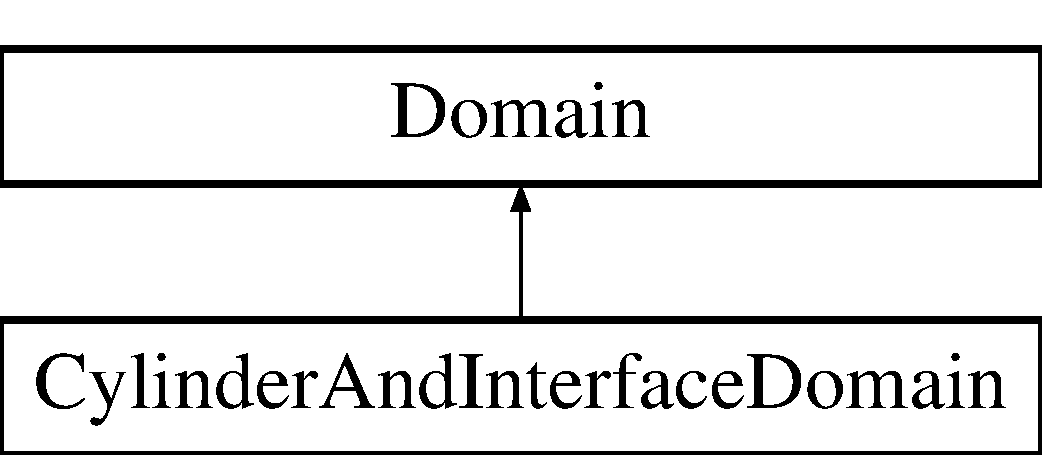
\includegraphics[height=2.000000cm]{classCylinderAndInterfaceDomain}
\end{center}
\end{figure}
\subsection*{Public Member Functions}
\begin{DoxyCompactItemize}
\item 
\hyperlink{classCylinderAndInterfaceDomain_a2025ff5337b4cb7889c26109857ed521}{Cylinder\+And\+Interface\+Domain} (const double \&Length, const double \&Height)
\item 
\hyperlink{classCylinderAndInterfaceDomain_aa204e83ef6332f121123465f4167d341}{$\sim$\+Cylinder\+And\+Interface\+Domain} ()
\item 
void \hyperlink{classCylinderAndInterfaceDomain_acab40651417c703e6b3dc592198c7497}{linear\+\_\+interpolate} (double Left\mbox{[}2\mbox{]}, double Right\mbox{[}2\mbox{]}, const double \&s, Vector$<$ double $>$ \&f)
\item 
void \hyperlink{classCylinderAndInterfaceDomain_a6afdef0d863b2833884aed2f571eeb79}{macro\+\_\+element\+\_\+boundary} (const unsigned \&time, const unsigned \&m, const unsigned \&direction, const Vector$<$ double $>$ \&s, Vector$<$ double $>$ \&f)
\end{DoxyCompactItemize}
\subsection*{Public Attributes}
\begin{DoxyCompactItemize}
\item 
double \hyperlink{classCylinderAndInterfaceDomain_a0b5aefe768267a1dff936ab491bee938}{centre\+\_\+x}
\item 
double \hyperlink{classCylinderAndInterfaceDomain_ac461297e0b08287a1909f245569c77f0}{centre\+\_\+y}
\end{DoxyCompactItemize}
\subsection*{Private Attributes}
\begin{DoxyCompactItemize}
\item 
double \hyperlink{classCylinderAndInterfaceDomain_a27c21e714221edda1d21995f941e74e3}{Lower\+\_\+left} \mbox{[}2\mbox{]}
\item 
double \hyperlink{classCylinderAndInterfaceDomain_a04206f6c72189356d5eecf32b81595f4}{Lower\+\_\+right} \mbox{[}2\mbox{]}
\item 
double \hyperlink{classCylinderAndInterfaceDomain_a5285785212f1cbcfb3910e87421d831c}{Lower\+\_\+mid\+\_\+left} \mbox{[}2\mbox{]}
\item 
double \hyperlink{classCylinderAndInterfaceDomain_a390ef76333ff22e7331b37ac7d5412bb}{Lower\+\_\+mid\+\_\+right} \mbox{[}2\mbox{]}
\item 
double \hyperlink{classCylinderAndInterfaceDomain_a2ad3d09d983dfcd5cc2a2b4c0d3d8b62}{Upper\+\_\+left} \mbox{[}2\mbox{]}
\item 
double \hyperlink{classCylinderAndInterfaceDomain_a87b1a618cc0116816b5460f00f3875a6}{Upper\+\_\+right} \mbox{[}2\mbox{]}
\item 
double \hyperlink{classCylinderAndInterfaceDomain_a01c924b854c98cb5a45ba2d1af43aa46}{Upper\+\_\+mid\+\_\+left} \mbox{[}2\mbox{]}
\item 
double \hyperlink{classCylinderAndInterfaceDomain_afb8019b28889f581f79541d571fb6386}{Upper\+\_\+mid\+\_\+right} \mbox{[}2\mbox{]}
\item 
double \hyperlink{classCylinderAndInterfaceDomain_a389bb3200199cf6098461f884e1b4d09}{Lower\+\_\+centre\+\_\+left} \mbox{[}2\mbox{]}
\item 
double \hyperlink{classCylinderAndInterfaceDomain_a1f1363c5343672e04be3b9f3285b0a25}{Lower\+\_\+centre\+\_\+right} \mbox{[}2\mbox{]}
\item 
double \hyperlink{classCylinderAndInterfaceDomain_a231d89466e433b65d0a6fd74b29b4609}{Upper\+\_\+centre\+\_\+left} \mbox{[}2\mbox{]}
\item 
double \hyperlink{classCylinderAndInterfaceDomain_a21972e49d0da0a5c1cbb89422b8bcfc3}{Upper\+\_\+centre\+\_\+right} \mbox{[}2\mbox{]}
\item 
Geom\+Object $\ast$ \hyperlink{classCylinderAndInterfaceDomain_aa0afda5d24ea33ff58957731e5b7dfd7}{Cylinder\+\_\+pt}
\begin{DoxyCompactList}\small\item\em Geometric object that represents the rotating cylinder. \end{DoxyCompactList}\end{DoxyCompactItemize}


\subsection{Detailed Description}


Definition at line 102 of file adaptive\+\_\+interface.\+cc.



\subsection{Constructor \& Destructor Documentation}
\mbox{\Hypertarget{classCylinderAndInterfaceDomain_a2025ff5337b4cb7889c26109857ed521}\label{classCylinderAndInterfaceDomain_a2025ff5337b4cb7889c26109857ed521}} 
\index{Cylinder\+And\+Interface\+Domain@{Cylinder\+And\+Interface\+Domain}!Cylinder\+And\+Interface\+Domain@{Cylinder\+And\+Interface\+Domain}}
\index{Cylinder\+And\+Interface\+Domain@{Cylinder\+And\+Interface\+Domain}!Cylinder\+And\+Interface\+Domain@{Cylinder\+And\+Interface\+Domain}}
\subsubsection{\texorpdfstring{Cylinder\+And\+Interface\+Domain()}{CylinderAndInterfaceDomain()}}
{\footnotesize\ttfamily Cylinder\+And\+Interface\+Domain\+::\+Cylinder\+And\+Interface\+Domain (\begin{DoxyParamCaption}\item[{const double \&}]{Length,  }\item[{const double \&}]{Height }\end{DoxyParamCaption})\hspace{0.3cm}{\ttfamily [inline]}}



Definition at line 121 of file adaptive\+\_\+interface.\+cc.

\mbox{\Hypertarget{classCylinderAndInterfaceDomain_aa204e83ef6332f121123465f4167d341}\label{classCylinderAndInterfaceDomain_aa204e83ef6332f121123465f4167d341}} 
\index{Cylinder\+And\+Interface\+Domain@{Cylinder\+And\+Interface\+Domain}!````~Cylinder\+And\+Interface\+Domain@{$\sim$\+Cylinder\+And\+Interface\+Domain}}
\index{````~Cylinder\+And\+Interface\+Domain@{$\sim$\+Cylinder\+And\+Interface\+Domain}!Cylinder\+And\+Interface\+Domain@{Cylinder\+And\+Interface\+Domain}}
\subsubsection{\texorpdfstring{$\sim$\+Cylinder\+And\+Interface\+Domain()}{~CylinderAndInterfaceDomain()}}
{\footnotesize\ttfamily Cylinder\+And\+Interface\+Domain\+::$\sim$\+Cylinder\+And\+Interface\+Domain (\begin{DoxyParamCaption}{ }\end{DoxyParamCaption})\hspace{0.3cm}{\ttfamily [inline]}}



Definition at line 193 of file adaptive\+\_\+interface.\+cc.



\subsection{Member Function Documentation}
\mbox{\Hypertarget{classCylinderAndInterfaceDomain_acab40651417c703e6b3dc592198c7497}\label{classCylinderAndInterfaceDomain_acab40651417c703e6b3dc592198c7497}} 
\index{Cylinder\+And\+Interface\+Domain@{Cylinder\+And\+Interface\+Domain}!linear\+\_\+interpolate@{linear\+\_\+interpolate}}
\index{linear\+\_\+interpolate@{linear\+\_\+interpolate}!Cylinder\+And\+Interface\+Domain@{Cylinder\+And\+Interface\+Domain}}
\subsubsection{\texorpdfstring{linear\+\_\+interpolate()}{linear\_interpolate()}}
{\footnotesize\ttfamily void Cylinder\+And\+Interface\+Domain\+::linear\+\_\+interpolate (\begin{DoxyParamCaption}\item[{double}]{Left\mbox{[}2\mbox{]},  }\item[{double}]{Right\mbox{[}2\mbox{]},  }\item[{const double \&}]{s,  }\item[{Vector$<$ double $>$ \&}]{f }\end{DoxyParamCaption})\hspace{0.3cm}{\ttfamily [inline]}}



Definition at line 200 of file adaptive\+\_\+interface.\+cc.

\mbox{\Hypertarget{classCylinderAndInterfaceDomain_a6afdef0d863b2833884aed2f571eeb79}\label{classCylinderAndInterfaceDomain_a6afdef0d863b2833884aed2f571eeb79}} 
\index{Cylinder\+And\+Interface\+Domain@{Cylinder\+And\+Interface\+Domain}!macro\+\_\+element\+\_\+boundary@{macro\+\_\+element\+\_\+boundary}}
\index{macro\+\_\+element\+\_\+boundary@{macro\+\_\+element\+\_\+boundary}!Cylinder\+And\+Interface\+Domain@{Cylinder\+And\+Interface\+Domain}}
\subsubsection{\texorpdfstring{macro\+\_\+element\+\_\+boundary()}{macro\_element\_boundary()}}
{\footnotesize\ttfamily void Cylinder\+And\+Interface\+Domain\+::macro\+\_\+element\+\_\+boundary (\begin{DoxyParamCaption}\item[{const unsigned \&}]{time,  }\item[{const unsigned \&}]{m,  }\item[{const unsigned \&}]{direction,  }\item[{const Vector$<$ double $>$ \&}]{s,  }\item[{Vector$<$ double $>$ \&}]{f }\end{DoxyParamCaption})\hspace{0.3cm}{\ttfamily [inline]}}



Definition at line 212 of file adaptive\+\_\+interface.\+cc.



\subsection{Member Data Documentation}
\mbox{\Hypertarget{classCylinderAndInterfaceDomain_a0b5aefe768267a1dff936ab491bee938}\label{classCylinderAndInterfaceDomain_a0b5aefe768267a1dff936ab491bee938}} 
\index{Cylinder\+And\+Interface\+Domain@{Cylinder\+And\+Interface\+Domain}!centre\+\_\+x@{centre\+\_\+x}}
\index{centre\+\_\+x@{centre\+\_\+x}!Cylinder\+And\+Interface\+Domain@{Cylinder\+And\+Interface\+Domain}}
\subsubsection{\texorpdfstring{centre\+\_\+x}{centre\_x}}
{\footnotesize\ttfamily double Cylinder\+And\+Interface\+Domain\+::centre\+\_\+x}



Definition at line 105 of file adaptive\+\_\+interface.\+cc.

\mbox{\Hypertarget{classCylinderAndInterfaceDomain_ac461297e0b08287a1909f245569c77f0}\label{classCylinderAndInterfaceDomain_ac461297e0b08287a1909f245569c77f0}} 
\index{Cylinder\+And\+Interface\+Domain@{Cylinder\+And\+Interface\+Domain}!centre\+\_\+y@{centre\+\_\+y}}
\index{centre\+\_\+y@{centre\+\_\+y}!Cylinder\+And\+Interface\+Domain@{Cylinder\+And\+Interface\+Domain}}
\subsubsection{\texorpdfstring{centre\+\_\+y}{centre\_y}}
{\footnotesize\ttfamily double Cylinder\+And\+Interface\+Domain\+::centre\+\_\+y}



Definition at line 105 of file adaptive\+\_\+interface.\+cc.

\mbox{\Hypertarget{classCylinderAndInterfaceDomain_aa0afda5d24ea33ff58957731e5b7dfd7}\label{classCylinderAndInterfaceDomain_aa0afda5d24ea33ff58957731e5b7dfd7}} 
\index{Cylinder\+And\+Interface\+Domain@{Cylinder\+And\+Interface\+Domain}!Cylinder\+\_\+pt@{Cylinder\+\_\+pt}}
\index{Cylinder\+\_\+pt@{Cylinder\+\_\+pt}!Cylinder\+And\+Interface\+Domain@{Cylinder\+And\+Interface\+Domain}}
\subsubsection{\texorpdfstring{Cylinder\+\_\+pt}{Cylinder\_pt}}
{\footnotesize\ttfamily Geom\+Object$\ast$ Cylinder\+And\+Interface\+Domain\+::\+Cylinder\+\_\+pt\hspace{0.3cm}{\ttfamily [private]}}



Geometric object that represents the rotating cylinder. 



Definition at line 116 of file adaptive\+\_\+interface.\+cc.

\mbox{\Hypertarget{classCylinderAndInterfaceDomain_a389bb3200199cf6098461f884e1b4d09}\label{classCylinderAndInterfaceDomain_a389bb3200199cf6098461f884e1b4d09}} 
\index{Cylinder\+And\+Interface\+Domain@{Cylinder\+And\+Interface\+Domain}!Lower\+\_\+centre\+\_\+left@{Lower\+\_\+centre\+\_\+left}}
\index{Lower\+\_\+centre\+\_\+left@{Lower\+\_\+centre\+\_\+left}!Cylinder\+And\+Interface\+Domain@{Cylinder\+And\+Interface\+Domain}}
\subsubsection{\texorpdfstring{Lower\+\_\+centre\+\_\+left}{Lower\_centre\_left}}
{\footnotesize\ttfamily double Cylinder\+And\+Interface\+Domain\+::\+Lower\+\_\+centre\+\_\+left\mbox{[}2\mbox{]}\hspace{0.3cm}{\ttfamily [private]}}



Definition at line 111 of file adaptive\+\_\+interface.\+cc.

\mbox{\Hypertarget{classCylinderAndInterfaceDomain_a1f1363c5343672e04be3b9f3285b0a25}\label{classCylinderAndInterfaceDomain_a1f1363c5343672e04be3b9f3285b0a25}} 
\index{Cylinder\+And\+Interface\+Domain@{Cylinder\+And\+Interface\+Domain}!Lower\+\_\+centre\+\_\+right@{Lower\+\_\+centre\+\_\+right}}
\index{Lower\+\_\+centre\+\_\+right@{Lower\+\_\+centre\+\_\+right}!Cylinder\+And\+Interface\+Domain@{Cylinder\+And\+Interface\+Domain}}
\subsubsection{\texorpdfstring{Lower\+\_\+centre\+\_\+right}{Lower\_centre\_right}}
{\footnotesize\ttfamily double Cylinder\+And\+Interface\+Domain\+::\+Lower\+\_\+centre\+\_\+right\mbox{[}2\mbox{]}\hspace{0.3cm}{\ttfamily [private]}}



Definition at line 111 of file adaptive\+\_\+interface.\+cc.

\mbox{\Hypertarget{classCylinderAndInterfaceDomain_a27c21e714221edda1d21995f941e74e3}\label{classCylinderAndInterfaceDomain_a27c21e714221edda1d21995f941e74e3}} 
\index{Cylinder\+And\+Interface\+Domain@{Cylinder\+And\+Interface\+Domain}!Lower\+\_\+left@{Lower\+\_\+left}}
\index{Lower\+\_\+left@{Lower\+\_\+left}!Cylinder\+And\+Interface\+Domain@{Cylinder\+And\+Interface\+Domain}}
\subsubsection{\texorpdfstring{Lower\+\_\+left}{Lower\_left}}
{\footnotesize\ttfamily double Cylinder\+And\+Interface\+Domain\+::\+Lower\+\_\+left\mbox{[}2\mbox{]}\hspace{0.3cm}{\ttfamily [private]}}



Definition at line 109 of file adaptive\+\_\+interface.\+cc.

\mbox{\Hypertarget{classCylinderAndInterfaceDomain_a5285785212f1cbcfb3910e87421d831c}\label{classCylinderAndInterfaceDomain_a5285785212f1cbcfb3910e87421d831c}} 
\index{Cylinder\+And\+Interface\+Domain@{Cylinder\+And\+Interface\+Domain}!Lower\+\_\+mid\+\_\+left@{Lower\+\_\+mid\+\_\+left}}
\index{Lower\+\_\+mid\+\_\+left@{Lower\+\_\+mid\+\_\+left}!Cylinder\+And\+Interface\+Domain@{Cylinder\+And\+Interface\+Domain}}
\subsubsection{\texorpdfstring{Lower\+\_\+mid\+\_\+left}{Lower\_mid\_left}}
{\footnotesize\ttfamily double Cylinder\+And\+Interface\+Domain\+::\+Lower\+\_\+mid\+\_\+left\mbox{[}2\mbox{]}\hspace{0.3cm}{\ttfamily [private]}}



Definition at line 109 of file adaptive\+\_\+interface.\+cc.

\mbox{\Hypertarget{classCylinderAndInterfaceDomain_a390ef76333ff22e7331b37ac7d5412bb}\label{classCylinderAndInterfaceDomain_a390ef76333ff22e7331b37ac7d5412bb}} 
\index{Cylinder\+And\+Interface\+Domain@{Cylinder\+And\+Interface\+Domain}!Lower\+\_\+mid\+\_\+right@{Lower\+\_\+mid\+\_\+right}}
\index{Lower\+\_\+mid\+\_\+right@{Lower\+\_\+mid\+\_\+right}!Cylinder\+And\+Interface\+Domain@{Cylinder\+And\+Interface\+Domain}}
\subsubsection{\texorpdfstring{Lower\+\_\+mid\+\_\+right}{Lower\_mid\_right}}
{\footnotesize\ttfamily double Cylinder\+And\+Interface\+Domain\+::\+Lower\+\_\+mid\+\_\+right\mbox{[}2\mbox{]}\hspace{0.3cm}{\ttfamily [private]}}



Definition at line 109 of file adaptive\+\_\+interface.\+cc.

\mbox{\Hypertarget{classCylinderAndInterfaceDomain_a04206f6c72189356d5eecf32b81595f4}\label{classCylinderAndInterfaceDomain_a04206f6c72189356d5eecf32b81595f4}} 
\index{Cylinder\+And\+Interface\+Domain@{Cylinder\+And\+Interface\+Domain}!Lower\+\_\+right@{Lower\+\_\+right}}
\index{Lower\+\_\+right@{Lower\+\_\+right}!Cylinder\+And\+Interface\+Domain@{Cylinder\+And\+Interface\+Domain}}
\subsubsection{\texorpdfstring{Lower\+\_\+right}{Lower\_right}}
{\footnotesize\ttfamily double Cylinder\+And\+Interface\+Domain\+::\+Lower\+\_\+right\mbox{[}2\mbox{]}\hspace{0.3cm}{\ttfamily [private]}}



Definition at line 109 of file adaptive\+\_\+interface.\+cc.

\mbox{\Hypertarget{classCylinderAndInterfaceDomain_a231d89466e433b65d0a6fd74b29b4609}\label{classCylinderAndInterfaceDomain_a231d89466e433b65d0a6fd74b29b4609}} 
\index{Cylinder\+And\+Interface\+Domain@{Cylinder\+And\+Interface\+Domain}!Upper\+\_\+centre\+\_\+left@{Upper\+\_\+centre\+\_\+left}}
\index{Upper\+\_\+centre\+\_\+left@{Upper\+\_\+centre\+\_\+left}!Cylinder\+And\+Interface\+Domain@{Cylinder\+And\+Interface\+Domain}}
\subsubsection{\texorpdfstring{Upper\+\_\+centre\+\_\+left}{Upper\_centre\_left}}
{\footnotesize\ttfamily double Cylinder\+And\+Interface\+Domain\+::\+Upper\+\_\+centre\+\_\+left\mbox{[}2\mbox{]}\hspace{0.3cm}{\ttfamily [private]}}



Definition at line 112 of file adaptive\+\_\+interface.\+cc.

\mbox{\Hypertarget{classCylinderAndInterfaceDomain_a21972e49d0da0a5c1cbb89422b8bcfc3}\label{classCylinderAndInterfaceDomain_a21972e49d0da0a5c1cbb89422b8bcfc3}} 
\index{Cylinder\+And\+Interface\+Domain@{Cylinder\+And\+Interface\+Domain}!Upper\+\_\+centre\+\_\+right@{Upper\+\_\+centre\+\_\+right}}
\index{Upper\+\_\+centre\+\_\+right@{Upper\+\_\+centre\+\_\+right}!Cylinder\+And\+Interface\+Domain@{Cylinder\+And\+Interface\+Domain}}
\subsubsection{\texorpdfstring{Upper\+\_\+centre\+\_\+right}{Upper\_centre\_right}}
{\footnotesize\ttfamily double Cylinder\+And\+Interface\+Domain\+::\+Upper\+\_\+centre\+\_\+right\mbox{[}2\mbox{]}\hspace{0.3cm}{\ttfamily [private]}}



Definition at line 112 of file adaptive\+\_\+interface.\+cc.

\mbox{\Hypertarget{classCylinderAndInterfaceDomain_a2ad3d09d983dfcd5cc2a2b4c0d3d8b62}\label{classCylinderAndInterfaceDomain_a2ad3d09d983dfcd5cc2a2b4c0d3d8b62}} 
\index{Cylinder\+And\+Interface\+Domain@{Cylinder\+And\+Interface\+Domain}!Upper\+\_\+left@{Upper\+\_\+left}}
\index{Upper\+\_\+left@{Upper\+\_\+left}!Cylinder\+And\+Interface\+Domain@{Cylinder\+And\+Interface\+Domain}}
\subsubsection{\texorpdfstring{Upper\+\_\+left}{Upper\_left}}
{\footnotesize\ttfamily double Cylinder\+And\+Interface\+Domain\+::\+Upper\+\_\+left\mbox{[}2\mbox{]}\hspace{0.3cm}{\ttfamily [private]}}



Definition at line 110 of file adaptive\+\_\+interface.\+cc.

\mbox{\Hypertarget{classCylinderAndInterfaceDomain_a01c924b854c98cb5a45ba2d1af43aa46}\label{classCylinderAndInterfaceDomain_a01c924b854c98cb5a45ba2d1af43aa46}} 
\index{Cylinder\+And\+Interface\+Domain@{Cylinder\+And\+Interface\+Domain}!Upper\+\_\+mid\+\_\+left@{Upper\+\_\+mid\+\_\+left}}
\index{Upper\+\_\+mid\+\_\+left@{Upper\+\_\+mid\+\_\+left}!Cylinder\+And\+Interface\+Domain@{Cylinder\+And\+Interface\+Domain}}
\subsubsection{\texorpdfstring{Upper\+\_\+mid\+\_\+left}{Upper\_mid\_left}}
{\footnotesize\ttfamily double Cylinder\+And\+Interface\+Domain\+::\+Upper\+\_\+mid\+\_\+left\mbox{[}2\mbox{]}\hspace{0.3cm}{\ttfamily [private]}}



Definition at line 110 of file adaptive\+\_\+interface.\+cc.

\mbox{\Hypertarget{classCylinderAndInterfaceDomain_afb8019b28889f581f79541d571fb6386}\label{classCylinderAndInterfaceDomain_afb8019b28889f581f79541d571fb6386}} 
\index{Cylinder\+And\+Interface\+Domain@{Cylinder\+And\+Interface\+Domain}!Upper\+\_\+mid\+\_\+right@{Upper\+\_\+mid\+\_\+right}}
\index{Upper\+\_\+mid\+\_\+right@{Upper\+\_\+mid\+\_\+right}!Cylinder\+And\+Interface\+Domain@{Cylinder\+And\+Interface\+Domain}}
\subsubsection{\texorpdfstring{Upper\+\_\+mid\+\_\+right}{Upper\_mid\_right}}
{\footnotesize\ttfamily double Cylinder\+And\+Interface\+Domain\+::\+Upper\+\_\+mid\+\_\+right\mbox{[}2\mbox{]}\hspace{0.3cm}{\ttfamily [private]}}



Definition at line 110 of file adaptive\+\_\+interface.\+cc.

\mbox{\Hypertarget{classCylinderAndInterfaceDomain_a87b1a618cc0116816b5460f00f3875a6}\label{classCylinderAndInterfaceDomain_a87b1a618cc0116816b5460f00f3875a6}} 
\index{Cylinder\+And\+Interface\+Domain@{Cylinder\+And\+Interface\+Domain}!Upper\+\_\+right@{Upper\+\_\+right}}
\index{Upper\+\_\+right@{Upper\+\_\+right}!Cylinder\+And\+Interface\+Domain@{Cylinder\+And\+Interface\+Domain}}
\subsubsection{\texorpdfstring{Upper\+\_\+right}{Upper\_right}}
{\footnotesize\ttfamily double Cylinder\+And\+Interface\+Domain\+::\+Upper\+\_\+right\mbox{[}2\mbox{]}\hspace{0.3cm}{\ttfamily [private]}}



Definition at line 110 of file adaptive\+\_\+interface.\+cc.



The documentation for this class was generated from the following file\+:\begin{DoxyCompactItemize}
\item 
\hyperlink{adaptive__interface_8cc}{adaptive\+\_\+interface.\+cc}\end{DoxyCompactItemize}

\hypertarget{classCylinderAndInterfaceMesh}{}\section{Cylinder\+And\+Interface\+Mesh$<$ E\+L\+E\+M\+E\+NT $>$ Class Template Reference}
\label{classCylinderAndInterfaceMesh}\index{Cylinder\+And\+Interface\+Mesh$<$ E\+L\+E\+M\+E\+N\+T $>$@{Cylinder\+And\+Interface\+Mesh$<$ E\+L\+E\+M\+E\+N\+T $>$}}
Inheritance diagram for Cylinder\+And\+Interface\+Mesh$<$ E\+L\+E\+M\+E\+NT $>$\+:\begin{figure}[H]
\begin{center}
\leavevmode
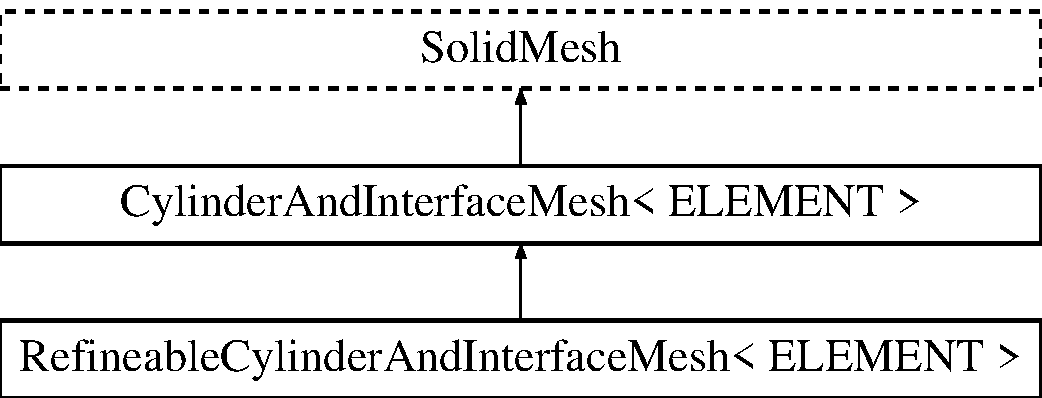
\includegraphics[height=3.000000cm]{classCylinderAndInterfaceMesh}
\end{center}
\end{figure}
\subsection*{Public Member Functions}
\begin{DoxyCompactItemize}
\item 
\hyperlink{classCylinderAndInterfaceDomain}{Cylinder\+And\+Interface\+Domain} $\ast$ \hyperlink{classCylinderAndInterfaceMesh_a924b3538d9f6c8b8524c317c5e2aa380}{domain\+\_\+pt} ()
\item 
\hyperlink{classCylinderAndInterfaceMesh_ab62eda41cc4a5516017b2662bcba8d17}{Cylinder\+And\+Interface\+Mesh} (const double \&length, const double \&height, Time\+Stepper $\ast$time\+\_\+stepper\+\_\+pt)
\end{DoxyCompactItemize}
\subsection*{Protected Attributes}
\begin{DoxyCompactItemize}
\item 
\hyperlink{classCylinderAndInterfaceDomain}{Cylinder\+And\+Interface\+Domain} $\ast$ \hyperlink{classCylinderAndInterfaceMesh_aa7b43c0cab4ffc92bb47813a8e255374}{Domain\+\_\+pt}
\end{DoxyCompactItemize}
\subsection*{Private Attributes}
\begin{DoxyCompactItemize}
\item 
double \hyperlink{classCylinderAndInterfaceMesh_a5ad81e65a9e9fb4c709a0c84f38216b1}{Height}
\end{DoxyCompactItemize}


\subsection{Detailed Description}
\subsubsection*{template$<$class E\+L\+E\+M\+E\+NT$>$\newline
class Cylinder\+And\+Interface\+Mesh$<$ E\+L\+E\+M\+E\+N\+T $>$}



Definition at line 446 of file adaptive\+\_\+interface.\+cc.



\subsection{Constructor \& Destructor Documentation}
\mbox{\Hypertarget{classCylinderAndInterfaceMesh_ab62eda41cc4a5516017b2662bcba8d17}\label{classCylinderAndInterfaceMesh_ab62eda41cc4a5516017b2662bcba8d17}} 
\index{Cylinder\+And\+Interface\+Mesh@{Cylinder\+And\+Interface\+Mesh}!Cylinder\+And\+Interface\+Mesh@{Cylinder\+And\+Interface\+Mesh}}
\index{Cylinder\+And\+Interface\+Mesh@{Cylinder\+And\+Interface\+Mesh}!Cylinder\+And\+Interface\+Mesh@{Cylinder\+And\+Interface\+Mesh}}
\subsubsection{\texorpdfstring{Cylinder\+And\+Interface\+Mesh()}{CylinderAndInterfaceMesh()}}
{\footnotesize\ttfamily template$<$class E\+L\+E\+M\+E\+NT $>$ \\
\hyperlink{classCylinderAndInterfaceMesh}{Cylinder\+And\+Interface\+Mesh}$<$ E\+L\+E\+M\+E\+NT $>$\+::\hyperlink{classCylinderAndInterfaceMesh}{Cylinder\+And\+Interface\+Mesh} (\begin{DoxyParamCaption}\item[{const double \&}]{length,  }\item[{const double \&}]{height,  }\item[{Time\+Stepper $\ast$}]{time\+\_\+stepper\+\_\+pt }\end{DoxyParamCaption})\hspace{0.3cm}{\ttfamily [inline]}}



Definition at line 460 of file adaptive\+\_\+interface.\+cc.



\subsection{Member Function Documentation}
\mbox{\Hypertarget{classCylinderAndInterfaceMesh_a924b3538d9f6c8b8524c317c5e2aa380}\label{classCylinderAndInterfaceMesh_a924b3538d9f6c8b8524c317c5e2aa380}} 
\index{Cylinder\+And\+Interface\+Mesh@{Cylinder\+And\+Interface\+Mesh}!domain\+\_\+pt@{domain\+\_\+pt}}
\index{domain\+\_\+pt@{domain\+\_\+pt}!Cylinder\+And\+Interface\+Mesh@{Cylinder\+And\+Interface\+Mesh}}
\subsubsection{\texorpdfstring{domain\+\_\+pt()}{domain\_pt()}}
{\footnotesize\ttfamily template$<$class E\+L\+E\+M\+E\+NT $>$ \\
\hyperlink{classCylinderAndInterfaceDomain}{Cylinder\+And\+Interface\+Domain}$\ast$ \hyperlink{classCylinderAndInterfaceMesh}{Cylinder\+And\+Interface\+Mesh}$<$ E\+L\+E\+M\+E\+NT $>$\+::domain\+\_\+pt (\begin{DoxyParamCaption}{ }\end{DoxyParamCaption})\hspace{0.3cm}{\ttfamily [inline]}}



Definition at line 457 of file adaptive\+\_\+interface.\+cc.



\subsection{Member Data Documentation}
\mbox{\Hypertarget{classCylinderAndInterfaceMesh_aa7b43c0cab4ffc92bb47813a8e255374}\label{classCylinderAndInterfaceMesh_aa7b43c0cab4ffc92bb47813a8e255374}} 
\index{Cylinder\+And\+Interface\+Mesh@{Cylinder\+And\+Interface\+Mesh}!Domain\+\_\+pt@{Domain\+\_\+pt}}
\index{Domain\+\_\+pt@{Domain\+\_\+pt}!Cylinder\+And\+Interface\+Mesh@{Cylinder\+And\+Interface\+Mesh}}
\subsubsection{\texorpdfstring{Domain\+\_\+pt}{Domain\_pt}}
{\footnotesize\ttfamily template$<$class E\+L\+E\+M\+E\+NT $>$ \\
\hyperlink{classCylinderAndInterfaceDomain}{Cylinder\+And\+Interface\+Domain}$\ast$ \hyperlink{classCylinderAndInterfaceMesh}{Cylinder\+And\+Interface\+Mesh}$<$ E\+L\+E\+M\+E\+NT $>$\+::Domain\+\_\+pt\hspace{0.3cm}{\ttfamily [protected]}}



Definition at line 452 of file adaptive\+\_\+interface.\+cc.

\mbox{\Hypertarget{classCylinderAndInterfaceMesh_a5ad81e65a9e9fb4c709a0c84f38216b1}\label{classCylinderAndInterfaceMesh_a5ad81e65a9e9fb4c709a0c84f38216b1}} 
\index{Cylinder\+And\+Interface\+Mesh@{Cylinder\+And\+Interface\+Mesh}!Height@{Height}}
\index{Height@{Height}!Cylinder\+And\+Interface\+Mesh@{Cylinder\+And\+Interface\+Mesh}}
\subsubsection{\texorpdfstring{Height}{Height}}
{\footnotesize\ttfamily template$<$class E\+L\+E\+M\+E\+NT $>$ \\
double \hyperlink{classCylinderAndInterfaceMesh}{Cylinder\+And\+Interface\+Mesh}$<$ E\+L\+E\+M\+E\+NT $>$\+::Height\hspace{0.3cm}{\ttfamily [private]}}



Definition at line 448 of file adaptive\+\_\+interface.\+cc.



The documentation for this class was generated from the following file\+:\begin{DoxyCompactItemize}
\item 
\hyperlink{adaptive__interface_8cc}{adaptive\+\_\+interface.\+cc}\end{DoxyCompactItemize}

\hypertarget{classGeneralEllipse}{}\section{General\+Ellipse Class Reference}
\label{classGeneralEllipse}\index{General\+Ellipse@{General\+Ellipse}}


A geometric object for an ellipse with initial centre of mass at (centre\+\_\+x, centre\+\_\+y) with axis in the x direction given by 2a and in the y-\/direction given by 2b. The boundary of the ellipse is parametrised by its angle.  


Inheritance diagram for General\+Ellipse\+:\begin{figure}[H]
\begin{center}
\leavevmode
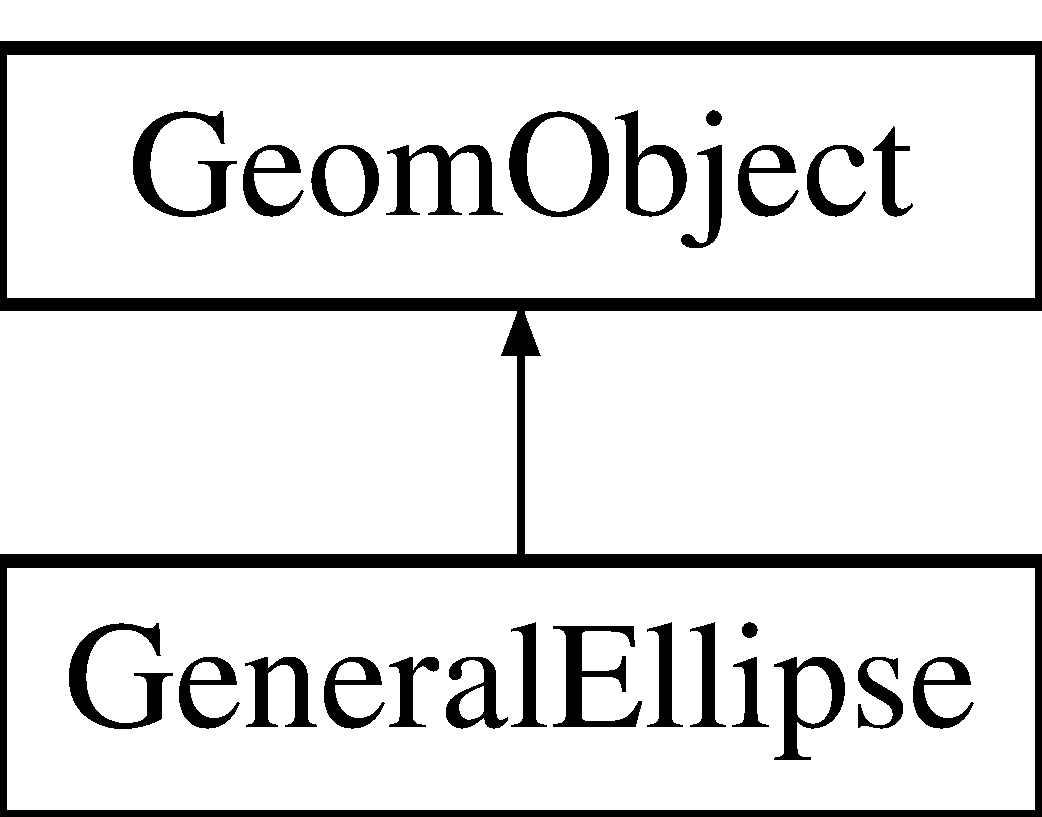
\includegraphics[height=2.000000cm]{classGeneralEllipse}
\end{center}
\end{figure}
\subsection*{Public Member Functions}
\begin{DoxyCompactItemize}
\item 
\hyperlink{classGeneralEllipse_a50dc036d709bcd1d53eafb62b5548f67}{General\+Ellipse} (const double \&centre\+\_\+x, const double \&centre\+\_\+y, const double \&a, const double \&b)
\begin{DoxyCompactList}\small\item\em Simple Constructor that transfers appropriate geometric parameters into internal data. \end{DoxyCompactList}\item 
\hyperlink{classGeneralEllipse_a3ac5c17cf8c4998f1b74913860cb3bb9}{$\sim$\+General\+Ellipse} ()
\begin{DoxyCompactList}\small\item\em Empty Destructor. \end{DoxyCompactList}\item 
void \hyperlink{classGeneralEllipse_a85e975c70441a9c9c711b5e27d124bff}{position} (const Vector$<$ double $>$ \&xi, Vector$<$ double $>$ \&r) const
\item 
void \hyperlink{classGeneralEllipse_a2bdcc69fcb1f1725124d625c032d171a}{position} (const unsigned \&t, const Vector$<$ double $>$ \&xi, Vector$<$ double $>$ \&r) const
\end{DoxyCompactItemize}
\subsection*{Private Attributes}
\begin{DoxyCompactItemize}
\item 
double \hyperlink{classGeneralEllipse_aeb974769f58d136a12ac1532506304cc}{Centre\+\_\+x}
\item 
double \hyperlink{classGeneralEllipse_abf2def5a5140bb35e381b800c4b91dc9}{Centre\+\_\+y}
\item 
double \hyperlink{classGeneralEllipse_ae583e1437da6ad4eb228dda60b61808a}{A}
\item 
double \hyperlink{classGeneralEllipse_a185ae9786d5c6c82eef61e163e9310c6}{B}
\end{DoxyCompactItemize}


\subsection{Detailed Description}
A geometric object for an ellipse with initial centre of mass at (centre\+\_\+x, centre\+\_\+y) with axis in the x direction given by 2a and in the y-\/direction given by 2b. The boundary of the ellipse is parametrised by its angle. 

Definition at line 149 of file jeffery\+\_\+orbit.\+cc.



\subsection{Constructor \& Destructor Documentation}
\mbox{\Hypertarget{classGeneralEllipse_a50dc036d709bcd1d53eafb62b5548f67}\label{classGeneralEllipse_a50dc036d709bcd1d53eafb62b5548f67}} 
\index{General\+Ellipse@{General\+Ellipse}!General\+Ellipse@{General\+Ellipse}}
\index{General\+Ellipse@{General\+Ellipse}!General\+Ellipse@{General\+Ellipse}}
\subsubsection{\texorpdfstring{General\+Ellipse()}{GeneralEllipse()}}
{\footnotesize\ttfamily General\+Ellipse\+::\+General\+Ellipse (\begin{DoxyParamCaption}\item[{const double \&}]{centre\+\_\+x,  }\item[{const double \&}]{centre\+\_\+y,  }\item[{const double \&}]{a,  }\item[{const double \&}]{b }\end{DoxyParamCaption})\hspace{0.3cm}{\ttfamily [inline]}}



Simple Constructor that transfers appropriate geometric parameters into internal data. 



Definition at line 160 of file jeffery\+\_\+orbit.\+cc.

\mbox{\Hypertarget{classGeneralEllipse_a3ac5c17cf8c4998f1b74913860cb3bb9}\label{classGeneralEllipse_a3ac5c17cf8c4998f1b74913860cb3bb9}} 
\index{General\+Ellipse@{General\+Ellipse}!````~General\+Ellipse@{$\sim$\+General\+Ellipse}}
\index{````~General\+Ellipse@{$\sim$\+General\+Ellipse}!General\+Ellipse@{General\+Ellipse}}
\subsubsection{\texorpdfstring{$\sim$\+General\+Ellipse()}{~GeneralEllipse()}}
{\footnotesize\ttfamily General\+Ellipse\+::$\sim$\+General\+Ellipse (\begin{DoxyParamCaption}{ }\end{DoxyParamCaption})\hspace{0.3cm}{\ttfamily [inline]}}



Empty Destructor. 



Definition at line 166 of file jeffery\+\_\+orbit.\+cc.



\subsection{Member Function Documentation}
\mbox{\Hypertarget{classGeneralEllipse_a85e975c70441a9c9c711b5e27d124bff}\label{classGeneralEllipse_a85e975c70441a9c9c711b5e27d124bff}} 
\index{General\+Ellipse@{General\+Ellipse}!position@{position}}
\index{position@{position}!General\+Ellipse@{General\+Ellipse}}
\subsubsection{\texorpdfstring{position()}{position()}\hspace{0.1cm}{\footnotesize\ttfamily [1/2]}}
{\footnotesize\ttfamily void General\+Ellipse\+::position (\begin{DoxyParamCaption}\item[{const Vector$<$ double $>$ \&}]{xi,  }\item[{Vector$<$ double $>$ \&}]{r }\end{DoxyParamCaption}) const\hspace{0.3cm}{\ttfamily [inline]}}

Return the position of the ellipse boundary as a function of the angle xi\mbox{[}0\mbox{]} 

Definition at line 170 of file jeffery\+\_\+orbit.\+cc.

\mbox{\Hypertarget{classGeneralEllipse_a2bdcc69fcb1f1725124d625c032d171a}\label{classGeneralEllipse_a2bdcc69fcb1f1725124d625c032d171a}} 
\index{General\+Ellipse@{General\+Ellipse}!position@{position}}
\index{position@{position}!General\+Ellipse@{General\+Ellipse}}
\subsubsection{\texorpdfstring{position()}{position()}\hspace{0.1cm}{\footnotesize\ttfamily [2/2]}}
{\footnotesize\ttfamily void General\+Ellipse\+::position (\begin{DoxyParamCaption}\item[{const unsigned \&}]{t,  }\item[{const Vector$<$ double $>$ \&}]{xi,  }\item[{Vector$<$ double $>$ \&}]{r }\end{DoxyParamCaption}) const\hspace{0.3cm}{\ttfamily [inline]}}



Definition at line 177 of file jeffery\+\_\+orbit.\+cc.



\subsection{Member Data Documentation}
\mbox{\Hypertarget{classGeneralEllipse_ae583e1437da6ad4eb228dda60b61808a}\label{classGeneralEllipse_ae583e1437da6ad4eb228dda60b61808a}} 
\index{General\+Ellipse@{General\+Ellipse}!A@{A}}
\index{A@{A}!General\+Ellipse@{General\+Ellipse}}
\subsubsection{\texorpdfstring{A}{A}}
{\footnotesize\ttfamily double General\+Ellipse\+::A\hspace{0.3cm}{\ttfamily [private]}}



Definition at line 154 of file jeffery\+\_\+orbit.\+cc.

\mbox{\Hypertarget{classGeneralEllipse_a185ae9786d5c6c82eef61e163e9310c6}\label{classGeneralEllipse_a185ae9786d5c6c82eef61e163e9310c6}} 
\index{General\+Ellipse@{General\+Ellipse}!B@{B}}
\index{B@{B}!General\+Ellipse@{General\+Ellipse}}
\subsubsection{\texorpdfstring{B}{B}}
{\footnotesize\ttfamily double General\+Ellipse\+::B\hspace{0.3cm}{\ttfamily [private]}}



Definition at line 154 of file jeffery\+\_\+orbit.\+cc.

\mbox{\Hypertarget{classGeneralEllipse_aeb974769f58d136a12ac1532506304cc}\label{classGeneralEllipse_aeb974769f58d136a12ac1532506304cc}} 
\index{General\+Ellipse@{General\+Ellipse}!Centre\+\_\+x@{Centre\+\_\+x}}
\index{Centre\+\_\+x@{Centre\+\_\+x}!General\+Ellipse@{General\+Ellipse}}
\subsubsection{\texorpdfstring{Centre\+\_\+x}{Centre\_x}}
{\footnotesize\ttfamily double General\+Ellipse\+::\+Centre\+\_\+x\hspace{0.3cm}{\ttfamily [private]}}



Definition at line 154 of file jeffery\+\_\+orbit.\+cc.

\mbox{\Hypertarget{classGeneralEllipse_abf2def5a5140bb35e381b800c4b91dc9}\label{classGeneralEllipse_abf2def5a5140bb35e381b800c4b91dc9}} 
\index{General\+Ellipse@{General\+Ellipse}!Centre\+\_\+y@{Centre\+\_\+y}}
\index{Centre\+\_\+y@{Centre\+\_\+y}!General\+Ellipse@{General\+Ellipse}}
\subsubsection{\texorpdfstring{Centre\+\_\+y}{Centre\_y}}
{\footnotesize\ttfamily double General\+Ellipse\+::\+Centre\+\_\+y\hspace{0.3cm}{\ttfamily [private]}}



Definition at line 154 of file jeffery\+\_\+orbit.\+cc.



The documentation for this class was generated from the following file\+:\begin{DoxyCompactItemize}
\item 
\hyperlink{jeffery__orbit_8cc}{jeffery\+\_\+orbit.\+cc}\end{DoxyCompactItemize}

\hypertarget{classRefineableCylinderAndInterfaceMesh}{}\section{Refineable\+Cylinder\+And\+Interface\+Mesh$<$ E\+L\+E\+M\+E\+NT $>$ Class Template Reference}
\label{classRefineableCylinderAndInterfaceMesh}\index{Refineable\+Cylinder\+And\+Interface\+Mesh$<$ E\+L\+E\+M\+E\+N\+T $>$@{Refineable\+Cylinder\+And\+Interface\+Mesh$<$ E\+L\+E\+M\+E\+N\+T $>$}}
Inheritance diagram for Refineable\+Cylinder\+And\+Interface\+Mesh$<$ E\+L\+E\+M\+E\+NT $>$\+:\begin{figure}[H]
\begin{center}
\leavevmode
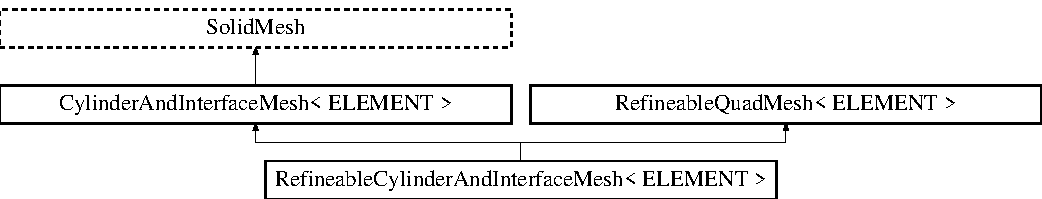
\includegraphics[height=2.675159cm]{classRefineableCylinderAndInterfaceMesh}
\end{center}
\end{figure}
\subsection*{Public Member Functions}
\begin{DoxyCompactItemize}
\item 
\hyperlink{classRefineableCylinderAndInterfaceMesh_a2f42954cee8f7ba47d87f842dbdc4cc2}{Refineable\+Cylinder\+And\+Interface\+Mesh} (const double \&length, const double \&height, Time\+Stepper $\ast$time\+\_\+stepper\+\_\+pt)
\item 
virtual \hyperlink{classRefineableCylinderAndInterfaceMesh_ad661ea3bc9100aaac36bc10aab9b2648}{$\sim$\+Refineable\+Cylinder\+And\+Interface\+Mesh} ()
\begin{DoxyCompactList}\small\item\em Destructor\+: Empty. \end{DoxyCompactList}\end{DoxyCompactItemize}
\subsection*{Additional Inherited Members}


\subsection{Detailed Description}
\subsubsection*{template$<$class E\+L\+E\+M\+E\+NT$>$\newline
class Refineable\+Cylinder\+And\+Interface\+Mesh$<$ E\+L\+E\+M\+E\+N\+T $>$}



Definition at line 693 of file adaptive\+\_\+interface.\+cc.



\subsection{Constructor \& Destructor Documentation}
\mbox{\Hypertarget{classRefineableCylinderAndInterfaceMesh_a2f42954cee8f7ba47d87f842dbdc4cc2}\label{classRefineableCylinderAndInterfaceMesh_a2f42954cee8f7ba47d87f842dbdc4cc2}} 
\index{Refineable\+Cylinder\+And\+Interface\+Mesh@{Refineable\+Cylinder\+And\+Interface\+Mesh}!Refineable\+Cylinder\+And\+Interface\+Mesh@{Refineable\+Cylinder\+And\+Interface\+Mesh}}
\index{Refineable\+Cylinder\+And\+Interface\+Mesh@{Refineable\+Cylinder\+And\+Interface\+Mesh}!Refineable\+Cylinder\+And\+Interface\+Mesh@{Refineable\+Cylinder\+And\+Interface\+Mesh}}
\subsubsection{\texorpdfstring{Refineable\+Cylinder\+And\+Interface\+Mesh()}{RefineableCylinderAndInterfaceMesh()}}
{\footnotesize\ttfamily template$<$class E\+L\+E\+M\+E\+NT$>$ \\
\hyperlink{classRefineableCylinderAndInterfaceMesh}{Refineable\+Cylinder\+And\+Interface\+Mesh}$<$ E\+L\+E\+M\+E\+NT $>$\+::\hyperlink{classRefineableCylinderAndInterfaceMesh}{Refineable\+Cylinder\+And\+Interface\+Mesh} (\begin{DoxyParamCaption}\item[{const double \&}]{length,  }\item[{const double \&}]{height,  }\item[{Time\+Stepper $\ast$}]{time\+\_\+stepper\+\_\+pt }\end{DoxyParamCaption})\hspace{0.3cm}{\ttfamily [inline]}}



Definition at line 699 of file adaptive\+\_\+interface.\+cc.

\mbox{\Hypertarget{classRefineableCylinderAndInterfaceMesh_ad661ea3bc9100aaac36bc10aab9b2648}\label{classRefineableCylinderAndInterfaceMesh_ad661ea3bc9100aaac36bc10aab9b2648}} 
\index{Refineable\+Cylinder\+And\+Interface\+Mesh@{Refineable\+Cylinder\+And\+Interface\+Mesh}!````~Refineable\+Cylinder\+And\+Interface\+Mesh@{$\sim$\+Refineable\+Cylinder\+And\+Interface\+Mesh}}
\index{````~Refineable\+Cylinder\+And\+Interface\+Mesh@{$\sim$\+Refineable\+Cylinder\+And\+Interface\+Mesh}!Refineable\+Cylinder\+And\+Interface\+Mesh@{Refineable\+Cylinder\+And\+Interface\+Mesh}}
\subsubsection{\texorpdfstring{$\sim$\+Refineable\+Cylinder\+And\+Interface\+Mesh()}{~RefineableCylinderAndInterfaceMesh()}}
{\footnotesize\ttfamily template$<$class E\+L\+E\+M\+E\+NT$>$ \\
virtual \hyperlink{classRefineableCylinderAndInterfaceMesh}{Refineable\+Cylinder\+And\+Interface\+Mesh}$<$ E\+L\+E\+M\+E\+NT $>$\+::$\sim$\hyperlink{classRefineableCylinderAndInterfaceMesh}{Refineable\+Cylinder\+And\+Interface\+Mesh} (\begin{DoxyParamCaption}{ }\end{DoxyParamCaption})\hspace{0.3cm}{\ttfamily [inline]}, {\ttfamily [virtual]}}



Destructor\+: Empty. 



Definition at line 724 of file adaptive\+\_\+interface.\+cc.



The documentation for this class was generated from the following file\+:\begin{DoxyCompactItemize}
\item 
\hyperlink{adaptive__interface_8cc}{adaptive\+\_\+interface.\+cc}\end{DoxyCompactItemize}

\hypertarget{classRefineableRotatingCylinderProblem}{}\section{Refineable\+Rotating\+Cylinder\+Problem$<$ E\+L\+E\+M\+E\+NT $>$ Class Template Reference}
\label{classRefineableRotatingCylinderProblem}\index{Refineable\+Rotating\+Cylinder\+Problem$<$ E\+L\+E\+M\+E\+N\+T $>$@{Refineable\+Rotating\+Cylinder\+Problem$<$ E\+L\+E\+M\+E\+N\+T $>$}}
Inheritance diagram for Refineable\+Rotating\+Cylinder\+Problem$<$ E\+L\+E\+M\+E\+NT $>$\+:\begin{figure}[H]
\begin{center}
\leavevmode
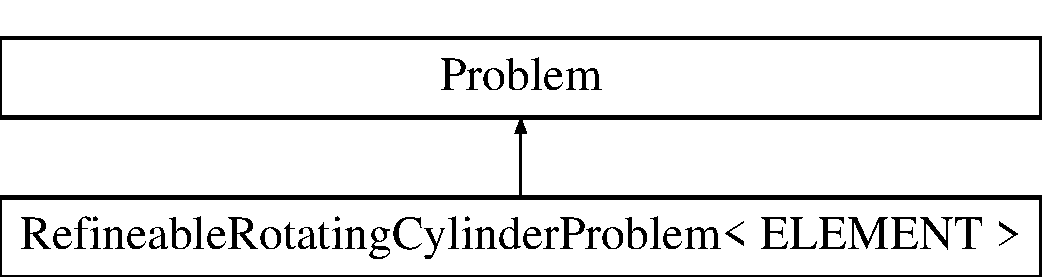
\includegraphics[height=2.000000cm]{classRefineableRotatingCylinderProblem}
\end{center}
\end{figure}
\subsection*{Public Member Functions}
\begin{DoxyCompactItemize}
\item 
\hyperlink{classRefineableRotatingCylinderProblem_aa597c4240ce9affbd7540998167c8f21}{Refineable\+Rotating\+Cylinder\+Problem} (const double \&length, const double \&height)
\item 
void \hyperlink{classRefineableRotatingCylinderProblem_af559552a0c8cba56b883cd8b5b283b7f}{actions\+\_\+after\+\_\+newton\+\_\+solve} ()
\begin{DoxyCompactList}\small\item\em Update the problem specs after solve (empty) \end{DoxyCompactList}\item 
void \hyperlink{classRefineableRotatingCylinderProblem_a382bc388316b410c45f337558b5ad577}{actions\+\_\+before\+\_\+newton\+\_\+solve} ()
\begin{DoxyCompactList}\small\item\em Update the problem specs before solve\+: \end{DoxyCompactList}\item 
void \hyperlink{classRefineableRotatingCylinderProblem_a705922ef2d96697ea5a110a412db5287}{actions\+\_\+before\+\_\+adapt} ()
\begin{DoxyCompactList}\small\item\em Strip off the interface before adaptation. \end{DoxyCompactList}\item 
void \hyperlink{classRefineableRotatingCylinderProblem_af914476e487ad5ed623384adb7c68c66}{actions\+\_\+after\+\_\+adapt} ()
\item 
void \hyperlink{classRefineableRotatingCylinderProblem_a417d18c2584ed1ea38daefe5dd68b4a4}{finish\+\_\+problem\+\_\+setup} ()
\begin{DoxyCompactList}\small\item\em Complete problem setup\+: Setup element-\/specific things (source fct pointers etc.) \end{DoxyCompactList}\item 
void \hyperlink{classRefineableRotatingCylinderProblem_acd510f2c06fa3f38d2911781656dbf20}{set\+\_\+boundary\+\_\+conditions} ()
\item 
void \hyperlink{classRefineableRotatingCylinderProblem_a664bfd373351a401619b06c3494fdcdc}{solve} ()
\item 
void \hyperlink{classRefineableRotatingCylinderProblem_a2de094b437cba9e9b71dca0afe587d65}{create\+\_\+volume\+\_\+constraint\+\_\+elements} ()
\begin{DoxyCompactList}\small\item\em Create the volume constraint elements. \end{DoxyCompactList}\item 
void \hyperlink{classRefineableRotatingCylinderProblem_a37cc1af7c83c5c1b7ae57f7f434be2f1}{delete\+\_\+volume\+\_\+constraint\+\_\+elements} ()
\item 
void \hyperlink{classRefineableRotatingCylinderProblem_a57623d36f2c97d300215c00ac917d449}{create\+\_\+free\+\_\+surface\+\_\+elements} ()
\item 
void \hyperlink{classRefineableRotatingCylinderProblem_ada026864153cf9954011bcea592cc5b7}{delete\+\_\+free\+\_\+surface\+\_\+elements} ()
\end{DoxyCompactItemize}
\subsection*{Public Attributes}
\begin{DoxyCompactItemize}
\item 
double \hyperlink{classRefineableRotatingCylinderProblem_a3a7fe3dd801eb1ef71dcf8e4c6a237ef}{Re}
\item 
double \hyperlink{classRefineableRotatingCylinderProblem_a2e47341fa1a71da29907ead94aeb5ec2}{Ca}
\item 
double \hyperlink{classRefineableRotatingCylinderProblem_acf70c93c4b4db46c1809f6b9f68214ee}{Re\+Inv\+Fr}
\item 
double \hyperlink{classRefineableRotatingCylinderProblem_a253a0d7954a3527bf1410f01080e5c70}{Bo}
\item 
double \hyperlink{classRefineableRotatingCylinderProblem_aaf1d39e57b4fc4d470b69f01121d93a3}{Omega}
\item 
double \hyperlink{classRefineableRotatingCylinderProblem_aa476013effb3f9a45cf1e1e2198aad14}{Volume}
\item 
double \hyperlink{classRefineableRotatingCylinderProblem_a54c8bf3a55597f50087c82ed5f955f5b}{Angle}
\item 
Vector$<$ double $>$ \hyperlink{classRefineableRotatingCylinderProblem_a270f2243978a54c8d787cc912168bb90}{G}
\item 
\hyperlink{classRefineableCylinderAndInterfaceMesh}{Refineable\+Cylinder\+And\+Interface\+Mesh}$<$ E\+L\+E\+M\+E\+NT $>$ $\ast$ \hyperlink{classRefineableRotatingCylinderProblem_aeb99a895bfdcceea6d13b41df7a59545}{Bulk\+\_\+mesh\+\_\+pt}
\item 
Mesh $\ast$ \hyperlink{classRefineableRotatingCylinderProblem_a48cc95921f8a03c220609d9666bcf406}{Surface\+\_\+mesh\+\_\+pt}
\item 
Mesh $\ast$ \hyperlink{classRefineableRotatingCylinderProblem_af438026e310576c522706dbff92ee750}{Point\+\_\+mesh\+\_\+pt}
\item 
Mesh $\ast$ \hyperlink{classRefineableRotatingCylinderProblem_a3bb79346179cb5ef1dad280530ea24e8}{Volume\+\_\+constraint\+\_\+mesh\+\_\+pt}
\begin{DoxyCompactList}\small\item\em The volume constraint mesh. \end{DoxyCompactList}\end{DoxyCompactItemize}
\subsection*{Private Attributes}
\begin{DoxyCompactItemize}
\item 
double \hyperlink{classRefineableRotatingCylinderProblem_acfa616d36346f557244146d4b2db9197}{Length}
\item 
double \hyperlink{classRefineableRotatingCylinderProblem_a3521efd0bfad036e20a6a8ba7e4547f4}{Height}
\item 
Constitutive\+Law $\ast$ \hyperlink{classRefineableRotatingCylinderProblem_a4e832fa2d6e1faafd39425d132d732e2}{Constitutive\+\_\+law\+\_\+pt}
\item 
Data $\ast$ \hyperlink{classRefineableRotatingCylinderProblem_a712d1cdcab28b62e1df830ffe1818009}{Traded\+\_\+pressure\+\_\+data\+\_\+pt}
\end{DoxyCompactItemize}


\subsection{Detailed Description}
\subsubsection*{template$<$class E\+L\+E\+M\+E\+NT$>$\newline
class Refineable\+Rotating\+Cylinder\+Problem$<$ E\+L\+E\+M\+E\+N\+T $>$}



Definition at line 730 of file adaptive\+\_\+interface.\+cc.



\subsection{Constructor \& Destructor Documentation}
\mbox{\Hypertarget{classRefineableRotatingCylinderProblem_aa597c4240ce9affbd7540998167c8f21}\label{classRefineableRotatingCylinderProblem_aa597c4240ce9affbd7540998167c8f21}} 
\index{Refineable\+Rotating\+Cylinder\+Problem@{Refineable\+Rotating\+Cylinder\+Problem}!Refineable\+Rotating\+Cylinder\+Problem@{Refineable\+Rotating\+Cylinder\+Problem}}
\index{Refineable\+Rotating\+Cylinder\+Problem@{Refineable\+Rotating\+Cylinder\+Problem}!Refineable\+Rotating\+Cylinder\+Problem@{Refineable\+Rotating\+Cylinder\+Problem}}
\subsubsection{\texorpdfstring{Refineable\+Rotating\+Cylinder\+Problem()}{RefineableRotatingCylinderProblem()}}
{\footnotesize\ttfamily template$<$class E\+L\+E\+M\+E\+NT $>$ \\
\hyperlink{classRefineableRotatingCylinderProblem}{Refineable\+Rotating\+Cylinder\+Problem}$<$ E\+L\+E\+M\+E\+NT $>$\+::\hyperlink{classRefineableRotatingCylinderProblem}{Refineable\+Rotating\+Cylinder\+Problem} (\begin{DoxyParamCaption}\item[{const double \&}]{length,  }\item[{const double \&}]{height }\end{DoxyParamCaption})}

Constructor\+: Pass flag to indicate if you want a constant source function or the tanh profile.

Constructor for adaptive Poisson problem in deformable fish-\/shaped domain. Pass bool to indicate if we want a constant source function or the one that produces a tanh step. Set the initial value of the Re\+Inv\+Fr = Bo/\+Ca

Build a linear solver\+: Use H\+SL\textquotesingle{}s M\+A42 frontal solver

Switch off full doc for frontal solver 

Definition at line 918 of file adaptive\+\_\+interface.\+cc.



References Refineable\+Rotating\+Cylinder\+Problem$<$ E\+L\+E\+M\+E\+N\+T $>$\+::\+Bo, Refineable\+Rotating\+Cylinder\+Problem$<$ E\+L\+E\+M\+E\+N\+T $>$\+::\+Bulk\+\_\+mesh\+\_\+pt, Refineable\+Rotating\+Cylinder\+Problem$<$ E\+L\+E\+M\+E\+N\+T $>$\+::\+Ca, Refineable\+Rotating\+Cylinder\+Problem$<$ E\+L\+E\+M\+E\+N\+T $>$\+::\+Constitutive\+\_\+law\+\_\+pt, Refineable\+Rotating\+Cylinder\+Problem$<$ E\+L\+E\+M\+E\+N\+T $>$\+::finish\+\_\+problem\+\_\+setup(), Refineable\+Rotating\+Cylinder\+Problem$<$ E\+L\+E\+M\+E\+N\+T $>$\+::G, Global\+\_\+\+Physical\+\_\+\+Variables\+::\+Nu, Refineable\+Rotating\+Cylinder\+Problem$<$ E\+L\+E\+M\+E\+N\+T $>$\+::\+Point\+\_\+mesh\+\_\+pt, Refineable\+Rotating\+Cylinder\+Problem$<$ E\+L\+E\+M\+E\+N\+T $>$\+::\+Re\+Inv\+Fr, Refineable\+Rotating\+Cylinder\+Problem$<$ E\+L\+E\+M\+E\+N\+T $>$\+::\+Surface\+\_\+mesh\+\_\+pt, Refineable\+Rotating\+Cylinder\+Problem$<$ E\+L\+E\+M\+E\+N\+T $>$\+::\+Traded\+\_\+pressure\+\_\+data\+\_\+pt, Refineable\+Rotating\+Cylinder\+Problem$<$ E\+L\+E\+M\+E\+N\+T $>$\+::\+Volume\+\_\+constraint\+\_\+mesh\+\_\+pt, and Global\+\_\+\+Physical\+\_\+\+Variables\+::\+Wall\+\_\+normal.



\subsection{Member Function Documentation}
\mbox{\Hypertarget{classRefineableRotatingCylinderProblem_af914476e487ad5ed623384adb7c68c66}\label{classRefineableRotatingCylinderProblem_af914476e487ad5ed623384adb7c68c66}} 
\index{Refineable\+Rotating\+Cylinder\+Problem@{Refineable\+Rotating\+Cylinder\+Problem}!actions\+\_\+after\+\_\+adapt@{actions\+\_\+after\+\_\+adapt}}
\index{actions\+\_\+after\+\_\+adapt@{actions\+\_\+after\+\_\+adapt}!Refineable\+Rotating\+Cylinder\+Problem@{Refineable\+Rotating\+Cylinder\+Problem}}
\subsubsection{\texorpdfstring{actions\+\_\+after\+\_\+adapt()}{actions\_after\_adapt()}}
{\footnotesize\ttfamily template$<$class E\+L\+E\+M\+E\+NT $>$ \\
void \hyperlink{classRefineableRotatingCylinderProblem}{Refineable\+Rotating\+Cylinder\+Problem}$<$ E\+L\+E\+M\+E\+NT $>$\+::actions\+\_\+after\+\_\+adapt (\begin{DoxyParamCaption}{ }\end{DoxyParamCaption})\hspace{0.3cm}{\ttfamily [inline]}}



Definition at line 769 of file adaptive\+\_\+interface.\+cc.

\mbox{\Hypertarget{classRefineableRotatingCylinderProblem_af559552a0c8cba56b883cd8b5b283b7f}\label{classRefineableRotatingCylinderProblem_af559552a0c8cba56b883cd8b5b283b7f}} 
\index{Refineable\+Rotating\+Cylinder\+Problem@{Refineable\+Rotating\+Cylinder\+Problem}!actions\+\_\+after\+\_\+newton\+\_\+solve@{actions\+\_\+after\+\_\+newton\+\_\+solve}}
\index{actions\+\_\+after\+\_\+newton\+\_\+solve@{actions\+\_\+after\+\_\+newton\+\_\+solve}!Refineable\+Rotating\+Cylinder\+Problem@{Refineable\+Rotating\+Cylinder\+Problem}}
\subsubsection{\texorpdfstring{actions\+\_\+after\+\_\+newton\+\_\+solve()}{actions\_after\_newton\_solve()}}
{\footnotesize\ttfamily template$<$class E\+L\+E\+M\+E\+NT $>$ \\
void \hyperlink{classRefineableRotatingCylinderProblem}{Refineable\+Rotating\+Cylinder\+Problem}$<$ E\+L\+E\+M\+E\+NT $>$\+::actions\+\_\+after\+\_\+newton\+\_\+solve (\begin{DoxyParamCaption}{ }\end{DoxyParamCaption})\hspace{0.3cm}{\ttfamily [inline]}}



Update the problem specs after solve (empty) 



Definition at line 757 of file adaptive\+\_\+interface.\+cc.

\mbox{\Hypertarget{classRefineableRotatingCylinderProblem_a705922ef2d96697ea5a110a412db5287}\label{classRefineableRotatingCylinderProblem_a705922ef2d96697ea5a110a412db5287}} 
\index{Refineable\+Rotating\+Cylinder\+Problem@{Refineable\+Rotating\+Cylinder\+Problem}!actions\+\_\+before\+\_\+adapt@{actions\+\_\+before\+\_\+adapt}}
\index{actions\+\_\+before\+\_\+adapt@{actions\+\_\+before\+\_\+adapt}!Refineable\+Rotating\+Cylinder\+Problem@{Refineable\+Rotating\+Cylinder\+Problem}}
\subsubsection{\texorpdfstring{actions\+\_\+before\+\_\+adapt()}{actions\_before\_adapt()}}
{\footnotesize\ttfamily template$<$class E\+L\+E\+M\+E\+NT $>$ \\
void \hyperlink{classRefineableRotatingCylinderProblem}{Refineable\+Rotating\+Cylinder\+Problem}$<$ E\+L\+E\+M\+E\+NT $>$\+::actions\+\_\+before\+\_\+adapt (\begin{DoxyParamCaption}{ }\end{DoxyParamCaption})\hspace{0.3cm}{\ttfamily [inline]}}



Strip off the interface before adaptation. 



Definition at line 763 of file adaptive\+\_\+interface.\+cc.

\mbox{\Hypertarget{classRefineableRotatingCylinderProblem_a382bc388316b410c45f337558b5ad577}\label{classRefineableRotatingCylinderProblem_a382bc388316b410c45f337558b5ad577}} 
\index{Refineable\+Rotating\+Cylinder\+Problem@{Refineable\+Rotating\+Cylinder\+Problem}!actions\+\_\+before\+\_\+newton\+\_\+solve@{actions\+\_\+before\+\_\+newton\+\_\+solve}}
\index{actions\+\_\+before\+\_\+newton\+\_\+solve@{actions\+\_\+before\+\_\+newton\+\_\+solve}!Refineable\+Rotating\+Cylinder\+Problem@{Refineable\+Rotating\+Cylinder\+Problem}}
\subsubsection{\texorpdfstring{actions\+\_\+before\+\_\+newton\+\_\+solve()}{actions\_before\_newton\_solve()}}
{\footnotesize\ttfamily template$<$class E\+L\+E\+M\+E\+NT $>$ \\
void \hyperlink{classRefineableRotatingCylinderProblem}{Refineable\+Rotating\+Cylinder\+Problem}$<$ E\+L\+E\+M\+E\+NT $>$\+::actions\+\_\+before\+\_\+newton\+\_\+solve (\begin{DoxyParamCaption}{ }\end{DoxyParamCaption})\hspace{0.3cm}{\ttfamily [inline]}}



Update the problem specs before solve\+: 



Definition at line 760 of file adaptive\+\_\+interface.\+cc.

\mbox{\Hypertarget{classRefineableRotatingCylinderProblem_a57623d36f2c97d300215c00ac917d449}\label{classRefineableRotatingCylinderProblem_a57623d36f2c97d300215c00ac917d449}} 
\index{Refineable\+Rotating\+Cylinder\+Problem@{Refineable\+Rotating\+Cylinder\+Problem}!create\+\_\+free\+\_\+surface\+\_\+elements@{create\+\_\+free\+\_\+surface\+\_\+elements}}
\index{create\+\_\+free\+\_\+surface\+\_\+elements@{create\+\_\+free\+\_\+surface\+\_\+elements}!Refineable\+Rotating\+Cylinder\+Problem@{Refineable\+Rotating\+Cylinder\+Problem}}
\subsubsection{\texorpdfstring{create\+\_\+free\+\_\+surface\+\_\+elements()}{create\_free\_surface\_elements()}}
{\footnotesize\ttfamily template$<$class E\+L\+E\+M\+E\+NT $>$ \\
void \hyperlink{classRefineableRotatingCylinderProblem}{Refineable\+Rotating\+Cylinder\+Problem}$<$ E\+L\+E\+M\+E\+NT $>$\+::create\+\_\+free\+\_\+surface\+\_\+elements (\begin{DoxyParamCaption}{ }\end{DoxyParamCaption})\hspace{0.3cm}{\ttfamily [inline]}}



Definition at line 840 of file adaptive\+\_\+interface.\+cc.



Referenced by Refineable\+Rotating\+Cylinder\+Problem$<$ E\+L\+E\+M\+E\+N\+T $>$\+::finish\+\_\+problem\+\_\+setup().

\mbox{\Hypertarget{classRefineableRotatingCylinderProblem_a2de094b437cba9e9b71dca0afe587d65}\label{classRefineableRotatingCylinderProblem_a2de094b437cba9e9b71dca0afe587d65}} 
\index{Refineable\+Rotating\+Cylinder\+Problem@{Refineable\+Rotating\+Cylinder\+Problem}!create\+\_\+volume\+\_\+constraint\+\_\+elements@{create\+\_\+volume\+\_\+constraint\+\_\+elements}}
\index{create\+\_\+volume\+\_\+constraint\+\_\+elements@{create\+\_\+volume\+\_\+constraint\+\_\+elements}!Refineable\+Rotating\+Cylinder\+Problem@{Refineable\+Rotating\+Cylinder\+Problem}}
\subsubsection{\texorpdfstring{create\+\_\+volume\+\_\+constraint\+\_\+elements()}{create\_volume\_constraint\_elements()}}
{\footnotesize\ttfamily template$<$class E\+L\+E\+M\+E\+NT $>$ \\
void \hyperlink{classRefineableRotatingCylinderProblem}{Refineable\+Rotating\+Cylinder\+Problem}$<$ E\+L\+E\+M\+E\+NT $>$\+::create\+\_\+volume\+\_\+constraint\+\_\+elements (\begin{DoxyParamCaption}{ }\end{DoxyParamCaption})\hspace{0.3cm}{\ttfamily [inline]}}



Create the volume constraint elements. 



Definition at line 792 of file adaptive\+\_\+interface.\+cc.



Referenced by Refineable\+Rotating\+Cylinder\+Problem$<$ E\+L\+E\+M\+E\+N\+T $>$\+::finish\+\_\+problem\+\_\+setup().

\mbox{\Hypertarget{classRefineableRotatingCylinderProblem_ada026864153cf9954011bcea592cc5b7}\label{classRefineableRotatingCylinderProblem_ada026864153cf9954011bcea592cc5b7}} 
\index{Refineable\+Rotating\+Cylinder\+Problem@{Refineable\+Rotating\+Cylinder\+Problem}!delete\+\_\+free\+\_\+surface\+\_\+elements@{delete\+\_\+free\+\_\+surface\+\_\+elements}}
\index{delete\+\_\+free\+\_\+surface\+\_\+elements@{delete\+\_\+free\+\_\+surface\+\_\+elements}!Refineable\+Rotating\+Cylinder\+Problem@{Refineable\+Rotating\+Cylinder\+Problem}}
\subsubsection{\texorpdfstring{delete\+\_\+free\+\_\+surface\+\_\+elements()}{delete\_free\_surface\_elements()}}
{\footnotesize\ttfamily template$<$class E\+L\+E\+M\+E\+NT $>$ \\
void \hyperlink{classRefineableRotatingCylinderProblem}{Refineable\+Rotating\+Cylinder\+Problem}$<$ E\+L\+E\+M\+E\+NT $>$\+::delete\+\_\+free\+\_\+surface\+\_\+elements (\begin{DoxyParamCaption}{ }\end{DoxyParamCaption})\hspace{0.3cm}{\ttfamily [inline]}}



Definition at line 891 of file adaptive\+\_\+interface.\+cc.

\mbox{\Hypertarget{classRefineableRotatingCylinderProblem_a37cc1af7c83c5c1b7ae57f7f434be2f1}\label{classRefineableRotatingCylinderProblem_a37cc1af7c83c5c1b7ae57f7f434be2f1}} 
\index{Refineable\+Rotating\+Cylinder\+Problem@{Refineable\+Rotating\+Cylinder\+Problem}!delete\+\_\+volume\+\_\+constraint\+\_\+elements@{delete\+\_\+volume\+\_\+constraint\+\_\+elements}}
\index{delete\+\_\+volume\+\_\+constraint\+\_\+elements@{delete\+\_\+volume\+\_\+constraint\+\_\+elements}!Refineable\+Rotating\+Cylinder\+Problem@{Refineable\+Rotating\+Cylinder\+Problem}}
\subsubsection{\texorpdfstring{delete\+\_\+volume\+\_\+constraint\+\_\+elements()}{delete\_volume\_constraint\_elements()}}
{\footnotesize\ttfamily template$<$class E\+L\+E\+M\+E\+NT $>$ \\
void \hyperlink{classRefineableRotatingCylinderProblem}{Refineable\+Rotating\+Cylinder\+Problem}$<$ E\+L\+E\+M\+E\+NT $>$\+::delete\+\_\+volume\+\_\+constraint\+\_\+elements (\begin{DoxyParamCaption}{ }\end{DoxyParamCaption})\hspace{0.3cm}{\ttfamily [inline]}}



Definition at line 830 of file adaptive\+\_\+interface.\+cc.

\mbox{\Hypertarget{classRefineableRotatingCylinderProblem_a417d18c2584ed1ea38daefe5dd68b4a4}\label{classRefineableRotatingCylinderProblem_a417d18c2584ed1ea38daefe5dd68b4a4}} 
\index{Refineable\+Rotating\+Cylinder\+Problem@{Refineable\+Rotating\+Cylinder\+Problem}!finish\+\_\+problem\+\_\+setup@{finish\+\_\+problem\+\_\+setup}}
\index{finish\+\_\+problem\+\_\+setup@{finish\+\_\+problem\+\_\+setup}!Refineable\+Rotating\+Cylinder\+Problem@{Refineable\+Rotating\+Cylinder\+Problem}}
\subsubsection{\texorpdfstring{finish\+\_\+problem\+\_\+setup()}{finish\_problem\_setup()}}
{\footnotesize\ttfamily template$<$class E\+L\+E\+M\+E\+NT $>$ \\
void \hyperlink{classRefineableRotatingCylinderProblem}{Refineable\+Rotating\+Cylinder\+Problem}$<$ E\+L\+E\+M\+E\+NT $>$\+::finish\+\_\+problem\+\_\+setup (\begin{DoxyParamCaption}{ }\end{DoxyParamCaption})}



Complete problem setup\+: Setup element-\/specific things (source fct pointers etc.) 

Complete build of Poisson problem\+: Loop over elements and setup pointers to source function. 

Definition at line 1009 of file adaptive\+\_\+interface.\+cc.



References Refineable\+Rotating\+Cylinder\+Problem$<$ E\+L\+E\+M\+E\+N\+T $>$\+::\+Angle, Refineable\+Rotating\+Cylinder\+Problem$<$ E\+L\+E\+M\+E\+N\+T $>$\+::\+Bulk\+\_\+mesh\+\_\+pt, Refineable\+Rotating\+Cylinder\+Problem$<$ E\+L\+E\+M\+E\+N\+T $>$\+::\+Ca, Refineable\+Rotating\+Cylinder\+Problem$<$ E\+L\+E\+M\+E\+N\+T $>$\+::\+Constitutive\+\_\+law\+\_\+pt, Refineable\+Rotating\+Cylinder\+Problem$<$ E\+L\+E\+M\+E\+N\+T $>$\+::create\+\_\+free\+\_\+surface\+\_\+elements(), Refineable\+Rotating\+Cylinder\+Problem$<$ E\+L\+E\+M\+E\+N\+T $>$\+::create\+\_\+volume\+\_\+constraint\+\_\+elements(), Refineable\+Rotating\+Cylinder\+Problem$<$ E\+L\+E\+M\+E\+N\+T $>$\+::G, Refineable\+Rotating\+Cylinder\+Problem$<$ E\+L\+E\+M\+E\+N\+T $>$\+::\+Point\+\_\+mesh\+\_\+pt, Refineable\+Rotating\+Cylinder\+Problem$<$ E\+L\+E\+M\+E\+N\+T $>$\+::\+Re, Refineable\+Rotating\+Cylinder\+Problem$<$ E\+L\+E\+M\+E\+N\+T $>$\+::\+Re\+Inv\+Fr, Refineable\+Rotating\+Cylinder\+Problem$<$ E\+L\+E\+M\+E\+N\+T $>$\+::\+Surface\+\_\+mesh\+\_\+pt, and Global\+\_\+\+Physical\+\_\+\+Variables\+::wall\+\_\+unit\+\_\+normal\+\_\+fct().



Referenced by Refineable\+Rotating\+Cylinder\+Problem$<$ E\+L\+E\+M\+E\+N\+T $>$\+::\+Refineable\+Rotating\+Cylinder\+Problem().

\mbox{\Hypertarget{classRefineableRotatingCylinderProblem_acd510f2c06fa3f38d2911781656dbf20}\label{classRefineableRotatingCylinderProblem_acd510f2c06fa3f38d2911781656dbf20}} 
\index{Refineable\+Rotating\+Cylinder\+Problem@{Refineable\+Rotating\+Cylinder\+Problem}!set\+\_\+boundary\+\_\+conditions@{set\+\_\+boundary\+\_\+conditions}}
\index{set\+\_\+boundary\+\_\+conditions@{set\+\_\+boundary\+\_\+conditions}!Refineable\+Rotating\+Cylinder\+Problem@{Refineable\+Rotating\+Cylinder\+Problem}}
\subsubsection{\texorpdfstring{set\+\_\+boundary\+\_\+conditions()}{set\_boundary\_conditions()}}
{\footnotesize\ttfamily template$<$class E\+L\+E\+M\+E\+NT $>$ \\
void \hyperlink{classRefineableRotatingCylinderProblem}{Refineable\+Rotating\+Cylinder\+Problem}$<$ E\+L\+E\+M\+E\+NT $>$\+::set\+\_\+boundary\+\_\+conditions (\begin{DoxyParamCaption}{ }\end{DoxyParamCaption})}



Definition at line 1145 of file adaptive\+\_\+interface.\+cc.



References Refineable\+Rotating\+Cylinder\+Problem$<$ E\+L\+E\+M\+E\+N\+T $>$\+::\+Bulk\+\_\+mesh\+\_\+pt, and Refineable\+Rotating\+Cylinder\+Problem$<$ E\+L\+E\+M\+E\+N\+T $>$\+::\+Omega.

\mbox{\Hypertarget{classRefineableRotatingCylinderProblem_a664bfd373351a401619b06c3494fdcdc}\label{classRefineableRotatingCylinderProblem_a664bfd373351a401619b06c3494fdcdc}} 
\index{Refineable\+Rotating\+Cylinder\+Problem@{Refineable\+Rotating\+Cylinder\+Problem}!solve@{solve}}
\index{solve@{solve}!Refineable\+Rotating\+Cylinder\+Problem@{Refineable\+Rotating\+Cylinder\+Problem}}
\subsubsection{\texorpdfstring{solve()}{solve()}}
{\footnotesize\ttfamily template$<$class E\+L\+E\+M\+E\+NT $>$ \\
void \hyperlink{classRefineableRotatingCylinderProblem}{Refineable\+Rotating\+Cylinder\+Problem}$<$ E\+L\+E\+M\+E\+NT $>$\+::solve (\begin{DoxyParamCaption}{ }\end{DoxyParamCaption})}



Definition at line 1170 of file adaptive\+\_\+interface.\+cc.



References Refineable\+Rotating\+Cylinder\+Problem$<$ E\+L\+E\+M\+E\+N\+T $>$\+::\+Angle, Refineable\+Rotating\+Cylinder\+Problem$<$ E\+L\+E\+M\+E\+N\+T $>$\+::\+Bulk\+\_\+mesh\+\_\+pt, Refineable\+Rotating\+Cylinder\+Problem$<$ E\+L\+E\+M\+E\+N\+T $>$\+::\+Ca, Refineable\+Rotating\+Cylinder\+Problem$<$ E\+L\+E\+M\+E\+N\+T $>$\+::\+Re\+Inv\+Fr, and Refineable\+Rotating\+Cylinder\+Problem$<$ E\+L\+E\+M\+E\+N\+T $>$\+::\+Surface\+\_\+mesh\+\_\+pt.



\subsection{Member Data Documentation}
\mbox{\Hypertarget{classRefineableRotatingCylinderProblem_a54c8bf3a55597f50087c82ed5f955f5b}\label{classRefineableRotatingCylinderProblem_a54c8bf3a55597f50087c82ed5f955f5b}} 
\index{Refineable\+Rotating\+Cylinder\+Problem@{Refineable\+Rotating\+Cylinder\+Problem}!Angle@{Angle}}
\index{Angle@{Angle}!Refineable\+Rotating\+Cylinder\+Problem@{Refineable\+Rotating\+Cylinder\+Problem}}
\subsubsection{\texorpdfstring{Angle}{Angle}}
{\footnotesize\ttfamily template$<$class E\+L\+E\+M\+E\+NT $>$ \\
double \hyperlink{classRefineableRotatingCylinderProblem}{Refineable\+Rotating\+Cylinder\+Problem}$<$ E\+L\+E\+M\+E\+NT $>$\+::Angle}



Definition at line 748 of file adaptive\+\_\+interface.\+cc.



Referenced by Refineable\+Rotating\+Cylinder\+Problem$<$ E\+L\+E\+M\+E\+N\+T $>$\+::finish\+\_\+problem\+\_\+setup(), and Refineable\+Rotating\+Cylinder\+Problem$<$ E\+L\+E\+M\+E\+N\+T $>$\+::solve().

\mbox{\Hypertarget{classRefineableRotatingCylinderProblem_a253a0d7954a3527bf1410f01080e5c70}\label{classRefineableRotatingCylinderProblem_a253a0d7954a3527bf1410f01080e5c70}} 
\index{Refineable\+Rotating\+Cylinder\+Problem@{Refineable\+Rotating\+Cylinder\+Problem}!Bo@{Bo}}
\index{Bo@{Bo}!Refineable\+Rotating\+Cylinder\+Problem@{Refineable\+Rotating\+Cylinder\+Problem}}
\subsubsection{\texorpdfstring{Bo}{Bo}}
{\footnotesize\ttfamily template$<$class E\+L\+E\+M\+E\+NT $>$ \\
double \hyperlink{classRefineableRotatingCylinderProblem}{Refineable\+Rotating\+Cylinder\+Problem}$<$ E\+L\+E\+M\+E\+NT $>$\+::Bo}



Definition at line 742 of file adaptive\+\_\+interface.\+cc.



Referenced by Refineable\+Rotating\+Cylinder\+Problem$<$ E\+L\+E\+M\+E\+N\+T $>$\+::\+Refineable\+Rotating\+Cylinder\+Problem().

\mbox{\Hypertarget{classRefineableRotatingCylinderProblem_aeb99a895bfdcceea6d13b41df7a59545}\label{classRefineableRotatingCylinderProblem_aeb99a895bfdcceea6d13b41df7a59545}} 
\index{Refineable\+Rotating\+Cylinder\+Problem@{Refineable\+Rotating\+Cylinder\+Problem}!Bulk\+\_\+mesh\+\_\+pt@{Bulk\+\_\+mesh\+\_\+pt}}
\index{Bulk\+\_\+mesh\+\_\+pt@{Bulk\+\_\+mesh\+\_\+pt}!Refineable\+Rotating\+Cylinder\+Problem@{Refineable\+Rotating\+Cylinder\+Problem}}
\subsubsection{\texorpdfstring{Bulk\+\_\+mesh\+\_\+pt}{Bulk\_mesh\_pt}}
{\footnotesize\ttfamily template$<$class E\+L\+E\+M\+E\+NT $>$ \\
\hyperlink{classRefineableCylinderAndInterfaceMesh}{Refineable\+Cylinder\+And\+Interface\+Mesh}$<$E\+L\+E\+M\+E\+NT$>$$\ast$ \hyperlink{classRefineableRotatingCylinderProblem}{Refineable\+Rotating\+Cylinder\+Problem}$<$ E\+L\+E\+M\+E\+NT $>$\+::Bulk\+\_\+mesh\+\_\+pt}



Definition at line 776 of file adaptive\+\_\+interface.\+cc.



Referenced by Refineable\+Rotating\+Cylinder\+Problem$<$ E\+L\+E\+M\+E\+N\+T $>$\+::finish\+\_\+problem\+\_\+setup(), Refineable\+Rotating\+Cylinder\+Problem$<$ E\+L\+E\+M\+E\+N\+T $>$\+::\+Refineable\+Rotating\+Cylinder\+Problem(), Refineable\+Rotating\+Cylinder\+Problem$<$ E\+L\+E\+M\+E\+N\+T $>$\+::set\+\_\+boundary\+\_\+conditions(), and Refineable\+Rotating\+Cylinder\+Problem$<$ E\+L\+E\+M\+E\+N\+T $>$\+::solve().

\mbox{\Hypertarget{classRefineableRotatingCylinderProblem_a2e47341fa1a71da29907ead94aeb5ec2}\label{classRefineableRotatingCylinderProblem_a2e47341fa1a71da29907ead94aeb5ec2}} 
\index{Refineable\+Rotating\+Cylinder\+Problem@{Refineable\+Rotating\+Cylinder\+Problem}!Ca@{Ca}}
\index{Ca@{Ca}!Refineable\+Rotating\+Cylinder\+Problem@{Refineable\+Rotating\+Cylinder\+Problem}}
\subsubsection{\texorpdfstring{Ca}{Ca}}
{\footnotesize\ttfamily template$<$class E\+L\+E\+M\+E\+NT $>$ \\
double \hyperlink{classRefineableRotatingCylinderProblem}{Refineable\+Rotating\+Cylinder\+Problem}$<$ E\+L\+E\+M\+E\+NT $>$\+::Ca}



Definition at line 742 of file adaptive\+\_\+interface.\+cc.



Referenced by Refineable\+Rotating\+Cylinder\+Problem$<$ E\+L\+E\+M\+E\+N\+T $>$\+::finish\+\_\+problem\+\_\+setup(), Refineable\+Rotating\+Cylinder\+Problem$<$ E\+L\+E\+M\+E\+N\+T $>$\+::\+Refineable\+Rotating\+Cylinder\+Problem(), and Refineable\+Rotating\+Cylinder\+Problem$<$ E\+L\+E\+M\+E\+N\+T $>$\+::solve().

\mbox{\Hypertarget{classRefineableRotatingCylinderProblem_a4e832fa2d6e1faafd39425d132d732e2}\label{classRefineableRotatingCylinderProblem_a4e832fa2d6e1faafd39425d132d732e2}} 
\index{Refineable\+Rotating\+Cylinder\+Problem@{Refineable\+Rotating\+Cylinder\+Problem}!Constitutive\+\_\+law\+\_\+pt@{Constitutive\+\_\+law\+\_\+pt}}
\index{Constitutive\+\_\+law\+\_\+pt@{Constitutive\+\_\+law\+\_\+pt}!Refineable\+Rotating\+Cylinder\+Problem@{Refineable\+Rotating\+Cylinder\+Problem}}
\subsubsection{\texorpdfstring{Constitutive\+\_\+law\+\_\+pt}{Constitutive\_law\_pt}}
{\footnotesize\ttfamily template$<$class E\+L\+E\+M\+E\+NT $>$ \\
Constitutive\+Law$\ast$ \hyperlink{classRefineableRotatingCylinderProblem}{Refineable\+Rotating\+Cylinder\+Problem}$<$ E\+L\+E\+M\+E\+NT $>$\+::Constitutive\+\_\+law\+\_\+pt\hspace{0.3cm}{\ttfamily [private]}}



Definition at line 736 of file adaptive\+\_\+interface.\+cc.



Referenced by Refineable\+Rotating\+Cylinder\+Problem$<$ E\+L\+E\+M\+E\+N\+T $>$\+::finish\+\_\+problem\+\_\+setup(), and Refineable\+Rotating\+Cylinder\+Problem$<$ E\+L\+E\+M\+E\+N\+T $>$\+::\+Refineable\+Rotating\+Cylinder\+Problem().

\mbox{\Hypertarget{classRefineableRotatingCylinderProblem_a270f2243978a54c8d787cc912168bb90}\label{classRefineableRotatingCylinderProblem_a270f2243978a54c8d787cc912168bb90}} 
\index{Refineable\+Rotating\+Cylinder\+Problem@{Refineable\+Rotating\+Cylinder\+Problem}!G@{G}}
\index{G@{G}!Refineable\+Rotating\+Cylinder\+Problem@{Refineable\+Rotating\+Cylinder\+Problem}}
\subsubsection{\texorpdfstring{G}{G}}
{\footnotesize\ttfamily template$<$class E\+L\+E\+M\+E\+NT $>$ \\
Vector$<$double$>$ \hyperlink{classRefineableRotatingCylinderProblem}{Refineable\+Rotating\+Cylinder\+Problem}$<$ E\+L\+E\+M\+E\+NT $>$\+::G}



Definition at line 750 of file adaptive\+\_\+interface.\+cc.



Referenced by Refineable\+Rotating\+Cylinder\+Problem$<$ E\+L\+E\+M\+E\+N\+T $>$\+::finish\+\_\+problem\+\_\+setup(), and Refineable\+Rotating\+Cylinder\+Problem$<$ E\+L\+E\+M\+E\+N\+T $>$\+::\+Refineable\+Rotating\+Cylinder\+Problem().

\mbox{\Hypertarget{classRefineableRotatingCylinderProblem_a3521efd0bfad036e20a6a8ba7e4547f4}\label{classRefineableRotatingCylinderProblem_a3521efd0bfad036e20a6a8ba7e4547f4}} 
\index{Refineable\+Rotating\+Cylinder\+Problem@{Refineable\+Rotating\+Cylinder\+Problem}!Height@{Height}}
\index{Height@{Height}!Refineable\+Rotating\+Cylinder\+Problem@{Refineable\+Rotating\+Cylinder\+Problem}}
\subsubsection{\texorpdfstring{Height}{Height}}
{\footnotesize\ttfamily template$<$class E\+L\+E\+M\+E\+NT $>$ \\
double \hyperlink{classRefineableRotatingCylinderProblem}{Refineable\+Rotating\+Cylinder\+Problem}$<$ E\+L\+E\+M\+E\+NT $>$\+::Height\hspace{0.3cm}{\ttfamily [private]}}



Definition at line 733 of file adaptive\+\_\+interface.\+cc.

\mbox{\Hypertarget{classRefineableRotatingCylinderProblem_acfa616d36346f557244146d4b2db9197}\label{classRefineableRotatingCylinderProblem_acfa616d36346f557244146d4b2db9197}} 
\index{Refineable\+Rotating\+Cylinder\+Problem@{Refineable\+Rotating\+Cylinder\+Problem}!Length@{Length}}
\index{Length@{Length}!Refineable\+Rotating\+Cylinder\+Problem@{Refineable\+Rotating\+Cylinder\+Problem}}
\subsubsection{\texorpdfstring{Length}{Length}}
{\footnotesize\ttfamily template$<$class E\+L\+E\+M\+E\+NT $>$ \\
double \hyperlink{classRefineableRotatingCylinderProblem}{Refineable\+Rotating\+Cylinder\+Problem}$<$ E\+L\+E\+M\+E\+NT $>$\+::Length\hspace{0.3cm}{\ttfamily [private]}}



Definition at line 733 of file adaptive\+\_\+interface.\+cc.

\mbox{\Hypertarget{classRefineableRotatingCylinderProblem_aaf1d39e57b4fc4d470b69f01121d93a3}\label{classRefineableRotatingCylinderProblem_aaf1d39e57b4fc4d470b69f01121d93a3}} 
\index{Refineable\+Rotating\+Cylinder\+Problem@{Refineable\+Rotating\+Cylinder\+Problem}!Omega@{Omega}}
\index{Omega@{Omega}!Refineable\+Rotating\+Cylinder\+Problem@{Refineable\+Rotating\+Cylinder\+Problem}}
\subsubsection{\texorpdfstring{Omega}{Omega}}
{\footnotesize\ttfamily template$<$class E\+L\+E\+M\+E\+NT $>$ \\
double \hyperlink{classRefineableRotatingCylinderProblem}{Refineable\+Rotating\+Cylinder\+Problem}$<$ E\+L\+E\+M\+E\+NT $>$\+::Omega}



Definition at line 744 of file adaptive\+\_\+interface.\+cc.



Referenced by Refineable\+Rotating\+Cylinder\+Problem$<$ E\+L\+E\+M\+E\+N\+T $>$\+::set\+\_\+boundary\+\_\+conditions().

\mbox{\Hypertarget{classRefineableRotatingCylinderProblem_af438026e310576c522706dbff92ee750}\label{classRefineableRotatingCylinderProblem_af438026e310576c522706dbff92ee750}} 
\index{Refineable\+Rotating\+Cylinder\+Problem@{Refineable\+Rotating\+Cylinder\+Problem}!Point\+\_\+mesh\+\_\+pt@{Point\+\_\+mesh\+\_\+pt}}
\index{Point\+\_\+mesh\+\_\+pt@{Point\+\_\+mesh\+\_\+pt}!Refineable\+Rotating\+Cylinder\+Problem@{Refineable\+Rotating\+Cylinder\+Problem}}
\subsubsection{\texorpdfstring{Point\+\_\+mesh\+\_\+pt}{Point\_mesh\_pt}}
{\footnotesize\ttfamily template$<$class E\+L\+E\+M\+E\+NT $>$ \\
Mesh$\ast$ \hyperlink{classRefineableRotatingCylinderProblem}{Refineable\+Rotating\+Cylinder\+Problem}$<$ E\+L\+E\+M\+E\+NT $>$\+::Point\+\_\+mesh\+\_\+pt}



Definition at line 782 of file adaptive\+\_\+interface.\+cc.



Referenced by Refineable\+Rotating\+Cylinder\+Problem$<$ E\+L\+E\+M\+E\+N\+T $>$\+::finish\+\_\+problem\+\_\+setup(), and Refineable\+Rotating\+Cylinder\+Problem$<$ E\+L\+E\+M\+E\+N\+T $>$\+::\+Refineable\+Rotating\+Cylinder\+Problem().

\mbox{\Hypertarget{classRefineableRotatingCylinderProblem_a3a7fe3dd801eb1ef71dcf8e4c6a237ef}\label{classRefineableRotatingCylinderProblem_a3a7fe3dd801eb1ef71dcf8e4c6a237ef}} 
\index{Refineable\+Rotating\+Cylinder\+Problem@{Refineable\+Rotating\+Cylinder\+Problem}!Re@{Re}}
\index{Re@{Re}!Refineable\+Rotating\+Cylinder\+Problem@{Refineable\+Rotating\+Cylinder\+Problem}}
\subsubsection{\texorpdfstring{Re}{Re}}
{\footnotesize\ttfamily template$<$class E\+L\+E\+M\+E\+NT $>$ \\
double \hyperlink{classRefineableRotatingCylinderProblem}{Refineable\+Rotating\+Cylinder\+Problem}$<$ E\+L\+E\+M\+E\+NT $>$\+::Re}



Definition at line 742 of file adaptive\+\_\+interface.\+cc.



Referenced by Refineable\+Rotating\+Cylinder\+Problem$<$ E\+L\+E\+M\+E\+N\+T $>$\+::finish\+\_\+problem\+\_\+setup().

\mbox{\Hypertarget{classRefineableRotatingCylinderProblem_acf70c93c4b4db46c1809f6b9f68214ee}\label{classRefineableRotatingCylinderProblem_acf70c93c4b4db46c1809f6b9f68214ee}} 
\index{Refineable\+Rotating\+Cylinder\+Problem@{Refineable\+Rotating\+Cylinder\+Problem}!Re\+Inv\+Fr@{Re\+Inv\+Fr}}
\index{Re\+Inv\+Fr@{Re\+Inv\+Fr}!Refineable\+Rotating\+Cylinder\+Problem@{Refineable\+Rotating\+Cylinder\+Problem}}
\subsubsection{\texorpdfstring{Re\+Inv\+Fr}{ReInvFr}}
{\footnotesize\ttfamily template$<$class E\+L\+E\+M\+E\+NT $>$ \\
double \hyperlink{classRefineableRotatingCylinderProblem}{Refineable\+Rotating\+Cylinder\+Problem}$<$ E\+L\+E\+M\+E\+NT $>$\+::Re\+Inv\+Fr}



Definition at line 742 of file adaptive\+\_\+interface.\+cc.



Referenced by Refineable\+Rotating\+Cylinder\+Problem$<$ E\+L\+E\+M\+E\+N\+T $>$\+::finish\+\_\+problem\+\_\+setup(), Refineable\+Rotating\+Cylinder\+Problem$<$ E\+L\+E\+M\+E\+N\+T $>$\+::\+Refineable\+Rotating\+Cylinder\+Problem(), and Refineable\+Rotating\+Cylinder\+Problem$<$ E\+L\+E\+M\+E\+N\+T $>$\+::solve().

\mbox{\Hypertarget{classRefineableRotatingCylinderProblem_a48cc95921f8a03c220609d9666bcf406}\label{classRefineableRotatingCylinderProblem_a48cc95921f8a03c220609d9666bcf406}} 
\index{Refineable\+Rotating\+Cylinder\+Problem@{Refineable\+Rotating\+Cylinder\+Problem}!Surface\+\_\+mesh\+\_\+pt@{Surface\+\_\+mesh\+\_\+pt}}
\index{Surface\+\_\+mesh\+\_\+pt@{Surface\+\_\+mesh\+\_\+pt}!Refineable\+Rotating\+Cylinder\+Problem@{Refineable\+Rotating\+Cylinder\+Problem}}
\subsubsection{\texorpdfstring{Surface\+\_\+mesh\+\_\+pt}{Surface\_mesh\_pt}}
{\footnotesize\ttfamily template$<$class E\+L\+E\+M\+E\+NT $>$ \\
Mesh$\ast$ \hyperlink{classRefineableRotatingCylinderProblem}{Refineable\+Rotating\+Cylinder\+Problem}$<$ E\+L\+E\+M\+E\+NT $>$\+::Surface\+\_\+mesh\+\_\+pt}



Definition at line 779 of file adaptive\+\_\+interface.\+cc.



Referenced by Refineable\+Rotating\+Cylinder\+Problem$<$ E\+L\+E\+M\+E\+N\+T $>$\+::finish\+\_\+problem\+\_\+setup(), Refineable\+Rotating\+Cylinder\+Problem$<$ E\+L\+E\+M\+E\+N\+T $>$\+::\+Refineable\+Rotating\+Cylinder\+Problem(), and Refineable\+Rotating\+Cylinder\+Problem$<$ E\+L\+E\+M\+E\+N\+T $>$\+::solve().

\mbox{\Hypertarget{classRefineableRotatingCylinderProblem_a712d1cdcab28b62e1df830ffe1818009}\label{classRefineableRotatingCylinderProblem_a712d1cdcab28b62e1df830ffe1818009}} 
\index{Refineable\+Rotating\+Cylinder\+Problem@{Refineable\+Rotating\+Cylinder\+Problem}!Traded\+\_\+pressure\+\_\+data\+\_\+pt@{Traded\+\_\+pressure\+\_\+data\+\_\+pt}}
\index{Traded\+\_\+pressure\+\_\+data\+\_\+pt@{Traded\+\_\+pressure\+\_\+data\+\_\+pt}!Refineable\+Rotating\+Cylinder\+Problem@{Refineable\+Rotating\+Cylinder\+Problem}}
\subsubsection{\texorpdfstring{Traded\+\_\+pressure\+\_\+data\+\_\+pt}{Traded\_pressure\_data\_pt}}
{\footnotesize\ttfamily template$<$class E\+L\+E\+M\+E\+NT $>$ \\
Data$\ast$ \hyperlink{classRefineableRotatingCylinderProblem}{Refineable\+Rotating\+Cylinder\+Problem}$<$ E\+L\+E\+M\+E\+NT $>$\+::Traded\+\_\+pressure\+\_\+data\+\_\+pt\hspace{0.3cm}{\ttfamily [private]}}



Definition at line 738 of file adaptive\+\_\+interface.\+cc.



Referenced by Refineable\+Rotating\+Cylinder\+Problem$<$ E\+L\+E\+M\+E\+N\+T $>$\+::\+Refineable\+Rotating\+Cylinder\+Problem().

\mbox{\Hypertarget{classRefineableRotatingCylinderProblem_aa476013effb3f9a45cf1e1e2198aad14}\label{classRefineableRotatingCylinderProblem_aa476013effb3f9a45cf1e1e2198aad14}} 
\index{Refineable\+Rotating\+Cylinder\+Problem@{Refineable\+Rotating\+Cylinder\+Problem}!Volume@{Volume}}
\index{Volume@{Volume}!Refineable\+Rotating\+Cylinder\+Problem@{Refineable\+Rotating\+Cylinder\+Problem}}
\subsubsection{\texorpdfstring{Volume}{Volume}}
{\footnotesize\ttfamily template$<$class E\+L\+E\+M\+E\+NT $>$ \\
double \hyperlink{classRefineableRotatingCylinderProblem}{Refineable\+Rotating\+Cylinder\+Problem}$<$ E\+L\+E\+M\+E\+NT $>$\+::Volume}



Definition at line 746 of file adaptive\+\_\+interface.\+cc.

\mbox{\Hypertarget{classRefineableRotatingCylinderProblem_a3bb79346179cb5ef1dad280530ea24e8}\label{classRefineableRotatingCylinderProblem_a3bb79346179cb5ef1dad280530ea24e8}} 
\index{Refineable\+Rotating\+Cylinder\+Problem@{Refineable\+Rotating\+Cylinder\+Problem}!Volume\+\_\+constraint\+\_\+mesh\+\_\+pt@{Volume\+\_\+constraint\+\_\+mesh\+\_\+pt}}
\index{Volume\+\_\+constraint\+\_\+mesh\+\_\+pt@{Volume\+\_\+constraint\+\_\+mesh\+\_\+pt}!Refineable\+Rotating\+Cylinder\+Problem@{Refineable\+Rotating\+Cylinder\+Problem}}
\subsubsection{\texorpdfstring{Volume\+\_\+constraint\+\_\+mesh\+\_\+pt}{Volume\_constraint\_mesh\_pt}}
{\footnotesize\ttfamily template$<$class E\+L\+E\+M\+E\+NT $>$ \\
Mesh$\ast$ \hyperlink{classRefineableRotatingCylinderProblem}{Refineable\+Rotating\+Cylinder\+Problem}$<$ E\+L\+E\+M\+E\+NT $>$\+::Volume\+\_\+constraint\+\_\+mesh\+\_\+pt}



The volume constraint mesh. 



Definition at line 785 of file adaptive\+\_\+interface.\+cc.



Referenced by Refineable\+Rotating\+Cylinder\+Problem$<$ E\+L\+E\+M\+E\+N\+T $>$\+::\+Refineable\+Rotating\+Cylinder\+Problem().



The documentation for this class was generated from the following file\+:\begin{DoxyCompactItemize}
\item 
\hyperlink{adaptive__interface_8cc}{adaptive\+\_\+interface.\+cc}\end{DoxyCompactItemize}

\chapter{File Documentation}
\hypertarget{adaptive__interface_8cc}{}\section{adaptive\+\_\+interface.\+cc File Reference}
\label{adaptive__interface_8cc}\index{adaptive\+\_\+interface.\+cc@{adaptive\+\_\+interface.\+cc}}
\subsection*{Classes}
\begin{DoxyCompactItemize}
\item 
class \hyperlink{classGeneralEllipse}{General\+Ellipse}
\item 
class \hyperlink{classCylinderAndInterfaceDomain}{Cylinder\+And\+Interface\+Domain}
\item 
class \hyperlink{classCylinderAndInterfaceMesh}{Cylinder\+And\+Interface\+Mesh$<$ E\+L\+E\+M\+E\+N\+T $>$}
\item 
class \hyperlink{classRefineableCylinderAndInterfaceMesh}{Refineable\+Cylinder\+And\+Interface\+Mesh$<$ E\+L\+E\+M\+E\+N\+T $>$}
\item 
class \hyperlink{classRefineableRotatingCylinderProblem}{Refineable\+Rotating\+Cylinder\+Problem$<$ E\+L\+E\+M\+E\+N\+T $>$}
\end{DoxyCompactItemize}
\subsection*{Namespaces}
\begin{DoxyCompactItemize}
\item 
 \hyperlink{namespaceGlobal__Physical__Variables}{Global\+\_\+\+Physical\+\_\+\+Variables}
\begin{DoxyCompactList}\small\item\em Namespace for physical parameters. \end{DoxyCompactList}\end{DoxyCompactItemize}
\subsection*{Functions}
\begin{DoxyCompactItemize}
\item 
void \hyperlink{namespaceGlobal__Physical__Variables_a0d48e8726fa485de2b2df2d5031ec41b}{Global\+\_\+\+Physical\+\_\+\+Variables\+::wall\+\_\+unit\+\_\+normal\+\_\+fct} (const Vector$<$ double $>$ \&x, Vector$<$ double $>$ \&normal)
\begin{DoxyCompactList}\small\item\em Function that specifies the wall unit normal. \end{DoxyCompactList}\item 
int \hyperlink{adaptive__interface_8cc_ae66f6b31b5ad750f1fe042a706a4e3d4}{main} ()
\end{DoxyCompactItemize}
\subsection*{Variables}
\begin{DoxyCompactItemize}
\item 
double \hyperlink{namespaceGlobal__Physical__Variables_a3962c36313826b19f216f6bbbdd6a477}{Global\+\_\+\+Physical\+\_\+\+Variables\+::\+Nu} =0.\+1
\begin{DoxyCompactList}\small\item\em Pseudo-\/solid Poisson ratio. \end{DoxyCompactList}\item 
Vector$<$ double $>$ \hyperlink{namespaceGlobal__Physical__Variables_a5feb3df21fc4a0adefadecb8a8ed98d7}{Global\+\_\+\+Physical\+\_\+\+Variables\+::\+Wall\+\_\+normal}
\begin{DoxyCompactList}\small\item\em Direction of the wall normal vector. \end{DoxyCompactList}\end{DoxyCompactItemize}


\subsection{Function Documentation}
\mbox{\Hypertarget{adaptive__interface_8cc_ae66f6b31b5ad750f1fe042a706a4e3d4}\label{adaptive__interface_8cc_ae66f6b31b5ad750f1fe042a706a4e3d4}} 
\index{adaptive\+\_\+interface.\+cc@{adaptive\+\_\+interface.\+cc}!main@{main}}
\index{main@{main}!adaptive\+\_\+interface.\+cc@{adaptive\+\_\+interface.\+cc}}
\subsubsection{\texorpdfstring{main()}{main()}}
{\footnotesize\ttfamily int main (\begin{DoxyParamCaption}{ }\end{DoxyParamCaption})}



Definition at line 1282 of file adaptive\+\_\+interface.\+cc.


\hypertarget{adaptive__interface_8txt__doxygenified_8h}{}\section{adaptive\+\_\+interface.\+txt\+\_\+doxygenified.\+h File Reference}
\label{adaptive__interface_8txt__doxygenified_8h}\index{adaptive\+\_\+interface.\+txt\+\_\+doxygenified.\+h@{adaptive\+\_\+interface.\+txt\+\_\+doxygenified.\+h}}

%--- End generated contents ---

% Index
\backmatter
\newpage
\phantomsection
\clearemptydoublepage
\addcontentsline{toc}{chapter}{Index}
\printindex

